%% uctest.tex 11/3/94
%% Copyright (C) 1988-2004 Daniel Gildea, BBF, Ethan Munson.
%
% This work may be distributed and/or modified under the
% conditions of the LaTeX Project Public License, either version 1.3
% of this license or (at your option) any later version.
% The latest version of this license is in
%   http://www.latex-project.org/lppl.txt
% and version 1.3 or later is part of all distributions of LaTeX
% version 2003/12/01 or later.
%
% This work has the LPPL maintenance status "maintained".
% 
% The Current Maintainer of this work is Daniel Gildea.
\documentclass[11pt]{ucthesis}
\setlength\parindent{0.5cm}

%% The graphicx package provides the includegraphics command.
\usepackage{graphicx}
\graphicspath{{../../../latex/graphics/}{./figures/}{./graphics/}}
%% The amssymb package provides various useful mathematical symbols
\usepackage{amssymb}
\usepackage{amsmath}
\usepackage{amsthm}
\usepackage{relsize} % \mathlarger
\usepackage{mathtools}
\usepackage{braket}
\usepackage{enumerate, enumitem}
\usepackage{caption}
\usepackage{subcaption}
\usepackage{float}
\usepackage{placeins} % something to do with figures not floating into next section
\usepackage{tikz}
\usetikzlibrary{arrows.meta}
% \usepackage[acronym,toc]{glosseries}

\usepackage[ruled,linesnumbered]{algorithm2e}
\usepackage[noend]{algpseudocode}
\usepackage{bbm}

\usepackage{etoolbox}
\AtBeginEnvironment{algorithm}{\ssp}
% \AtBeginEnvironment{figure}{\ssp}
\AtBeginEnvironment{equation}{\ssp}
\AtBeginEnvironment{thebibliography}{\ssp}

\usepackage[linktocpage=true]{hyperref}
\newcommand\mycommfont[1]{\footnotesize\ttfamily\textcolor{black}{#1}}
\SetCommentSty{mycommfont}

\makeatletter
\def\BState{\State\hskip-\ALG@thistlm}
\makeatother

\newcommand{\edge}{%
  \mathrel{-}% minus as a relation
  \joinrel\joinrel % some backup
  \mathrel{-}% minus as a relation
}
\newcommand{\notedge}{%
  \mathrel{\mkern2mu}% a small advancement
  \arrownot % a short slash
  \mathrel{\mkern-2mu}% compensate
  \edge
}

\def\dsp{\def\baselinestretch{2.0}\large\normalsize}
\dsp

\newcommand{\vect}[1]{{\it{\boldsymbol{#1}}}}

\DeclareMathOperator*{\argmax}{arg\,max}
\DeclareMathOperator*{\argmin}{arg\,min}

\begin{document}
% Declarations for Front Matter

\title{Autonomous Field Exploration Using Prediction Variance Suppression}
\author{Sargis S Yonan}
\degreeyear{2018}
\degreemonth{December}
\degree{MASTER OF SCIENCE}
\chair{Professor Gabriel Hugh Elkaim}
\committeememberone{Professor Renwick E. Curry}
\committeemembertwo{Professor Patrick E. Mantey}
\numberofmembers{3} %% (including chair) possible: 3, 4, 5, 6
\deanlineone{Lori Kletzer}
\deanlinetwo{Vice Provost and Dean of Graduate Studies}
\deanlinethree{}
\field{COMPUTER ENGINEERING}
\emphasis{ROBOTICS AND CONTROL}
\campus{Santa Cruz}

\begin{frontmatter}

\maketitle
\copyrightpage

\tableofcontents
\listoffigures
% \listoftables

\end{frontmatter}


\begin{abstract}

A set of methods and path planners are introduced for the exploration of unknown semi-to-fully-ergodic fields of interest using an autonomous exploration vehicle with turn and speed control. The spatial statistical properties of a target field can be exploited to assist in variance suppressing planning techniques from observations of a single state of interest. The Kriging Method, a \textit{Best Linear Unbiased Predictor}, is used to exploit the statistical properties, namely the spatial autocorrelation, of a target field. The Kriging Method predicts the state of unobserved points from a set of observed points for the purposes of quality mapping. A prediction and confidence of prediction of the entirety of a given target field can be generated from the method.

The path planners introduced can be used to reduce the overall prediction uncertainty of a field by steering a single vehicle to collect a good set of samples. A metric for return on investment of executing a trajectory using feedback from Kriging predictions is presented. The three path planners introduced suppress the overall uncertainty of a Kriging prediction of an unknown target field in order to create a higher quality map when compared to a preplanned scanning regime, and another Kriging variance suppressing method (Greedy Next-Best-View), for the same distance traveled.

\end{abstract}

\begin{dedication}
\null\vfil
{\large
\begin{center}

TODO
% For my mother, Marina

\vspace{12pt}
\end{center}}
\vfil\null
\end{dedication}

\begin{acknowledgements}

TODO

% \noindent To my colleagues in The Autonomous Systems Lab at UC Santa Cruz, namely: Sharon Rabinovich, Renwick E. Curry, Gabriel Hugh Elkaim, Pavlo Vlastos, and Jordan Liss.\\

% \noindent To Space Exploration Technologies (SpaceX) for allowing me to participate on their mission to Mars, and for inspiring me to gear my field exploration method toward the exploration of the red planet.\\

\end{acknowledgements}


\chapter{Introduction}
% Why is this problem important? 
% We are introducing the concept of aerial field exploration
Field exploration is a method in which an unknown field (a \textit{target field}) is learned in an attempt to discover traits or track trends about the field. Field exploration methods can be useful for tracking the health of crop soil, the size of ice glaciers, generating terrain maps, and a wide variety of scientific, agricultural, and industrial purposes. Furthermore, an exploration technique, versus a patrolling or tracking technique where a target is tracked or surveilled, does not require a model of the target field dynamics, as they can be learned on-the-fly. A variety of fields can be explored without the knowledge of the initial values, or model, of the state of interest being observed in the field.

%% for some real life examples, we are going to argue why UAVs are the medium in which we should choose for our explorations
Using an Unmanned Aerial Vehicle (UAV) system, for example, an unknown field of interest can be scanned within a more reasonable time frame compared to conventional scanning techniques involving satellite and manned-airplane missions. Potentially more nuanced data can be gathered from the UAV made observations because of more desirable fields of view and more customizable sensors on-board. Using the techniques introduced, a high-quality map can be generated of a previously unknown field of interest. Satellite imagery of Earth has been used for measuring various natural phenomena in the past several decades. Estimating polar ice cap melting rates and exploring the location of an oil spills are among the class of problems solved by this technology. Currently, using a service like the US Forest Services' Moderate Resolution Imaging Spectroradiometer (MODIS) Active Fire Mapping Program, images are updated every 1 to 2 days with a fixed sensor. While this program is helpful for detecting large events with long periods of activity, the sampling rate of this service might not give an emergency response team or a scientist the required resolution and precision in gathered data at their desired rate. The resolution and frequency problem along with the cost associated with building, launching, and maintaining an orbiting Earth satellite might even make some areas of research prohibitive. The use of unmanned aerial vehicles (UAVs) have more recently been used in similar fields of study and in environmental protection. The benefits gained from using UAVs is that of more rapidly acquired data with more easily adjusted accuracy. A UAV can give more nuanced and detailed data on features of a field that are not observable from the distance or field of view of an orbiting satellite. This is because the UAV can be equipped with any compatible sensor and can be deployed from virtually anywhere to fly virtually anywhere.

% What have others done before me? How is what I'm doing different? Why is it better?
Presently, a common approach to exploring a field is to conduct a zig-zag pattern, or other predetermined maneuver on a target field. This task might take longer than needed to collect the required data, and could potentially ineffectively use the flight or drive time of the exploration vehicle which often has a short and limited runtime. A method that exploits the learned stochastic properties of a field could be used to decrease exploration time by avoiding the need to scan more points than needed. A majority of the unobserved points in a field can be predicted to a known degree of confidence, given a degree of spatial autocorrelation in the field. Furthermore, scanning every point in a large unknown field is an unrealistic expectation for vehicles with limited maneuvering capabilities. This is especially a problem if the field as a whole is very large and needs to only be predicted to a small degree of confidence. A scheme for minimal and high-quality scanning via variance suppressing path planning would be in the benefit of time for the user(s) of such a system, and the scanning equipment as well.

By exploiting the Kriging variances generated by the predictions from a set of samples taken on a field, variance based path planning methods can be used to steer an exploration vehicle in the areas of maximal uncertainty, while traversing over other areas of low prediction confidence. The methods introduced attempt to help a user of this system explore an unknown field with a known degree of confidence that is configurable through a desired runtime, tuned by the user.

\section{Previous Works}
The goal of this thesis is to introduce path planning techniques which reduce overall uncertainty of Kriging field predictions by steering a single vehicle through a field optimally. Using Kriging predictions as feedback into a path planner, to estimate confidence return for a given trajectory, is introduced in this work. Previous works have discussed autonomous field exploration in terms of predetermined sampling paths, or slightly dynamically selected paths. The use of Kriging variances in a path planner in a publication, when this work was originally started, did not exist. Near the completion of this thesis, a paper discussing the benefits of using Kriging variance motivated path planning for field exploration, was published \cite{fentanes:soilkrig}.

Exploration is a subset of the types of missions UAVs have been used for recently. From Section 2 of Nikhil Nigam's \textit{The Multiple Unmanned Air Vehicle Persistent Surveillance Problem: A Review} \cite{nigam:missions}, the various types of missions possible are described. There exist problems of tracking and patrolling which involve following a moving target, or of finding the spread rate and source of an item of interest. The exploration mission type is a procedure which runs parallel to the these types of missions. Without a model describing the states of the item of interest being explored, a simple scanning procedure involving random movements or following a predetermined path, like a zig-zag about the field as in \cite{semsch:uav_zig} are executed, or a zig-zag which incorporates the model dynamics of the vehicle, as in \cite{nigam:zigzag}. In \textit{Autonomous Aeromagnetic Surveys Using a Fluxgate Magnetometer} by Douglas G. Macharet et al., A UAV is used in a mineral field exploration technique, where a fluxgate sensor is used to measure the magnetic flux of a vesicle beneath the UAV \cite{macharet:magnet}. A zig-zag pattern is ultimately used to explore the field for minerals of interest. A more dynamic strategy is used in the autonomous home vacuum cleaner \textit{Roomba} by iRobot, where a spiral pattern is used in an attempt to clean up and find the periphery of debris \cite{roomba:spiral}. The radius of the spiral pattern is a function of the amount of debris tracked by the debris sensor in the immediate area of the vacuum cleaner.

Exploration missions often do not specify the model of the item of interest being tracked. Knowing the model and kinematics of the item being tracked makes it possible to use an optimal estimation tool such as an Extended Kalman Filter as in Rabinovich et al. \textit{A Methodology For Estimation of Ground Phenomena Propagation} \cite{sharon:uav_est} and \textit{Multi-UAV Path Coordination Based on Uncertainty Estimation} \cite{sharon:uav_uncert} where the velocity and position states of a ground fire are estimated while tracking the points surrounding the periphery of a wildfire. The planner for this mission calculates a path based off of the Kalman variances of the control points representing the periphery of the ground phenomenon being tracked. Variance based path planning is used in the path planners introduced in this thesis in Chapter \ref{ch:pp}.

The Kriging Method has been used in a UAV Contour Tracking problem in Zhang et al. \textit{Oil Spills Boundary Tracking Using Universal Kriging And Model Predictive Control By UAV} \cite{zhang:oil_krig}. The work relies on the knowledge of a model of the oil spill, and therefore is not a generic case of an exploration problem of a model-less field.

C. C. Castello et al. present the use of the Kriging method for environmental sensor placement in \textit{Optimal Sensor Placement Strategy for Environmental Monitoring using Wireless Sensor Networks} \cite{kriging:sensorplacement}. The overall variances of a Kriging predicted field, predicted from a set measurements from fixed sensor locations, can be directly compared to the variances of predicting the same field with a different set of sensor locations. The method can therefore be used to help assist in optimal sensor placement by conducting a Monte Carlo simulation of random sensor placements, and ultimately choosing the random configuration that minimized the Kriging prediction variances for the field. A path planner, which can be stated as a sensor placement problem, by selecting a random path, or set of sampling locations, that minimizes the expected Kriging variance of a target field is introduced in this thesis in Section \ref{sec:mcpp}. The use of a Monte Carlo approach, where noise is used to assist in suppressing prediction uncertainty has been used for uncertainty suppression in obstacle avoidance motion planning in \textit{Monte Carlo Motion Planning for Robot Trajectory Optimization Under Uncertainty} \cite{janson:mcmp}, but the technique is not used for exploration purposes, as introduced in this thesis.

While nearing completion of this thesis, Pulido Fentanes et al. published \textit{Kriging-Based Robotic Exploration for Soil Moisture Mapping Using a Cosmic-Ray Sensor}, where a Kriging variance based exploration technique is used for the purpose of quality mapping of agricultural soil moisture \cite{fentanes:soilkrig}. In the publication, three Kriging variance motivated path planners are used to reduce Kriging prediction error by steering an agricultural robot into areas of high Kriging variance. The first of their path planners, named \textit{Greedy Next-Best-View} (NBV), similar to the \textit{Next Highest Variance} (NHV) strategy demonstrated in this thesis, simply targets the highest variance on the Kriging variance field. In the Greedy NBV algorithm, the path is recalculated every time the robot takes a sample. In NHV, a path is only recalculated when the last endpoint (the highest variance of the last Kriging calculation of the field) is met. The authors of the publication also introduce a \textit{Monte Carlo Next-Best-View} where a set of random endpoints are generated and weighted against one another according to their Kriging variances. The endpoint that yields the point of highest uncertainty is ultimately selected as the next sample location. In this thesis, a Monte Carlo technique is also introduced in Section \ref{sec:mcpp}, but instead of weighing each proposed random trajectory by its Kriging variance, the predicted values of the points along a random trajectory are plugged back into the sampled field, and a Kriging variance calculation is run on the field again. The path that is ultimately chosen in this proposed planner, is the path which reduces the expected overall Kriging variance of the field as a whole. Lastly, the authors introduce an adaptive sampling planner which works by generating an initial path that is then modified after each sample taken. As more possible path are generated randomly, points get removed from the possible set of endpoints when their Kriging variance falls below the mean of the variance field. This method considers the mission time and minimum expectation of the measurement quality by re-planning and using a Traveling Salesperson (TSP) algorithm. In this thesis, minimum expected measurement quality is set before an exploration by tuning the maximum allowed area to scan.
\section{Problem Definitions} \label{ch:defs}
The problem space will be defined in an effort to be consistent in naming conventions and parameter definitions throughout this work. The conventions described in Section \ref{ch:defs} will be used throughout the rest of the work.

\subsection{Notation}
A boldface lowercase letter, for example, $\vect{v}$, will denote a column vector of real numbers. An non-boldface uppercase letter, for example, $M$, will denote a two-dimensional matrix of real numbers.

\subsection{The Field}
The initially unknown field, referred to as the \textit{target field}, is a rectangular field of height $h$, and width $w$, i.e. $Z \in \mathbb{R}^{h \times w}$. The field is made up of square pixel cells, referred to as \textit{vesicles}. Each vesicle can be ``visited'', or sampled, in order to yield a single state of interest in the set of real numbers. Throughout this thesis a square target field (i.e. $h = w$) will be used, and $h$ and $w$ will be natural numbers.

\subsection{The Sensor} \label{sec:sensor_measurements}
The observations of interest made on the field will be using ideal sensors with no measurement noise. The sensors will measure a subset of the area of the entire target field. This area will be referred to as the \textit{sensor footprint}, and will be equal to the size of a single vesicle of the target field.

The locations of the sensor measurements must be known for the methods developed. The locations of the measurements will be represented as Cartesian coordinates on the field. For an arbitrary observation of the field, the location of the measurement will be at corresponding coordinates $\vect{s} \in \mathbb{R}^2$, and the  sensor measurement would be $Z(\vect{s})$. The value of $Z$ at $\vect{s}$ is quantized to the vesicle in which the point $\vect{s}$ falls within.

\subsubsection{Real World Sensing Examples}
A Global Positioning System (GPS) sensor would likely be used to estimate localized position of a sensor measurement on Earth. In the case of predicting the boundaries of a glacier, for example, an infrared sensor would likely be used to measure the state of interest, thermal output of the field in this case. In the case of terrain mapping a LiDAR sensor could be used to sample terrain altitudes of the terrain below, at marked locations using GPS, on a UAV.



% \part{Background}
% \part{Spatial Analysis}
\chapter{Introduction to The Kriging Method}
Many of the methods introduced will rely on works developed in the fields of Spatial Statistics, Geostatistics, and Geography. Geo-statisticians have developed much of the work surrounding field predictions in the geospatial domain. In an effort to make the methods introduced be as presentable and contained as possible, a background on the required tools from the field of geostatistics will be reviewed. The Kriging Method, a best linear unbiased predictor (BLUP), and the heart of the method introduced, produces a prediction based on statistical data gathered from samples taken on a field. The method performs a weighted least squares on weights from a covariance matrix created from points sampled on a field. A variance for each prediction computed can also generated as a byproduct of the Kriging prediction, and will be used to calculate information gain in a path finder introduced in this paper. The assumption that the expected value of each point is from a normal distribution, where the variance and expected value of the distribution is a function of geospatial autocorrelation, will be used.

Tobler's First Law of Geography \cite{tobler:first_law} states,``Everything is related to everything else, but near things are more related than distant things." Regarding geospatial data, there is a positive correlation between observations with a small difference in distance \cite{miller:on_toblers_first_law}. This implies the existence of geospatial autocorrelation in many target fields of interest. This implies a positive correlation between elements in the spatial series that are of interest to the introduced technique. Geospatial autocorrelation is the hypothesis that allows naive prediction techniques, like Inverse Distance Weighting (IDW) (Section \ref{sec:idw_intro}), to work. 

Furthermore, if the target fields are viewed as an unknown spatial stochastic process, with a generally known underlying Gaussian statistical model (Guassian kernel), more weight in the Inverse Distance Weighting can be placed on the geospatial elements more related to the point that one desires to predict. A best linear unbiased predictor, like The Kriging Method, does just that by first finding the underlying spatial pattern of the field, and then predicting. The methods introduced in this chapter are intended to serve as an introduction to the Kriging Method, and aerial geospatial field interpolation in general.

\subsection{Autocorrelation in a Field}
Positively correlated geospatial autocorrelation in a field implies the existence of a cluster of similar points near one another i.e. relatively small covariances between two spatially similar points. The opposite is true when the overall geospatial autocorrelation of a field is negative. Using Tobler's First Law of Geography, the assumption that fields measured will contain positive autocorrelation will be used. The degree of geospatial autocorrelation in a field can be measured, and will be discussed in Section \ref{sec:vario} on Variography.

\begin{figure}[ht!]
    \centering
    \begin{subfigure}[t]{0.5\textwidth}
        \centering
        \includegraphics[width=\linewidth]{figures/generated_field.png}
        \captionsetup{skip=0.5\baselineskip,size=footnotesize}
        \caption{A randomly generated geospatially autocorrelated field.}
		\label{fig:gen_field}
    \end{subfigure}%
    ~ 
    \begin{subfigure}[t]{0.5\textwidth}
        \centering
        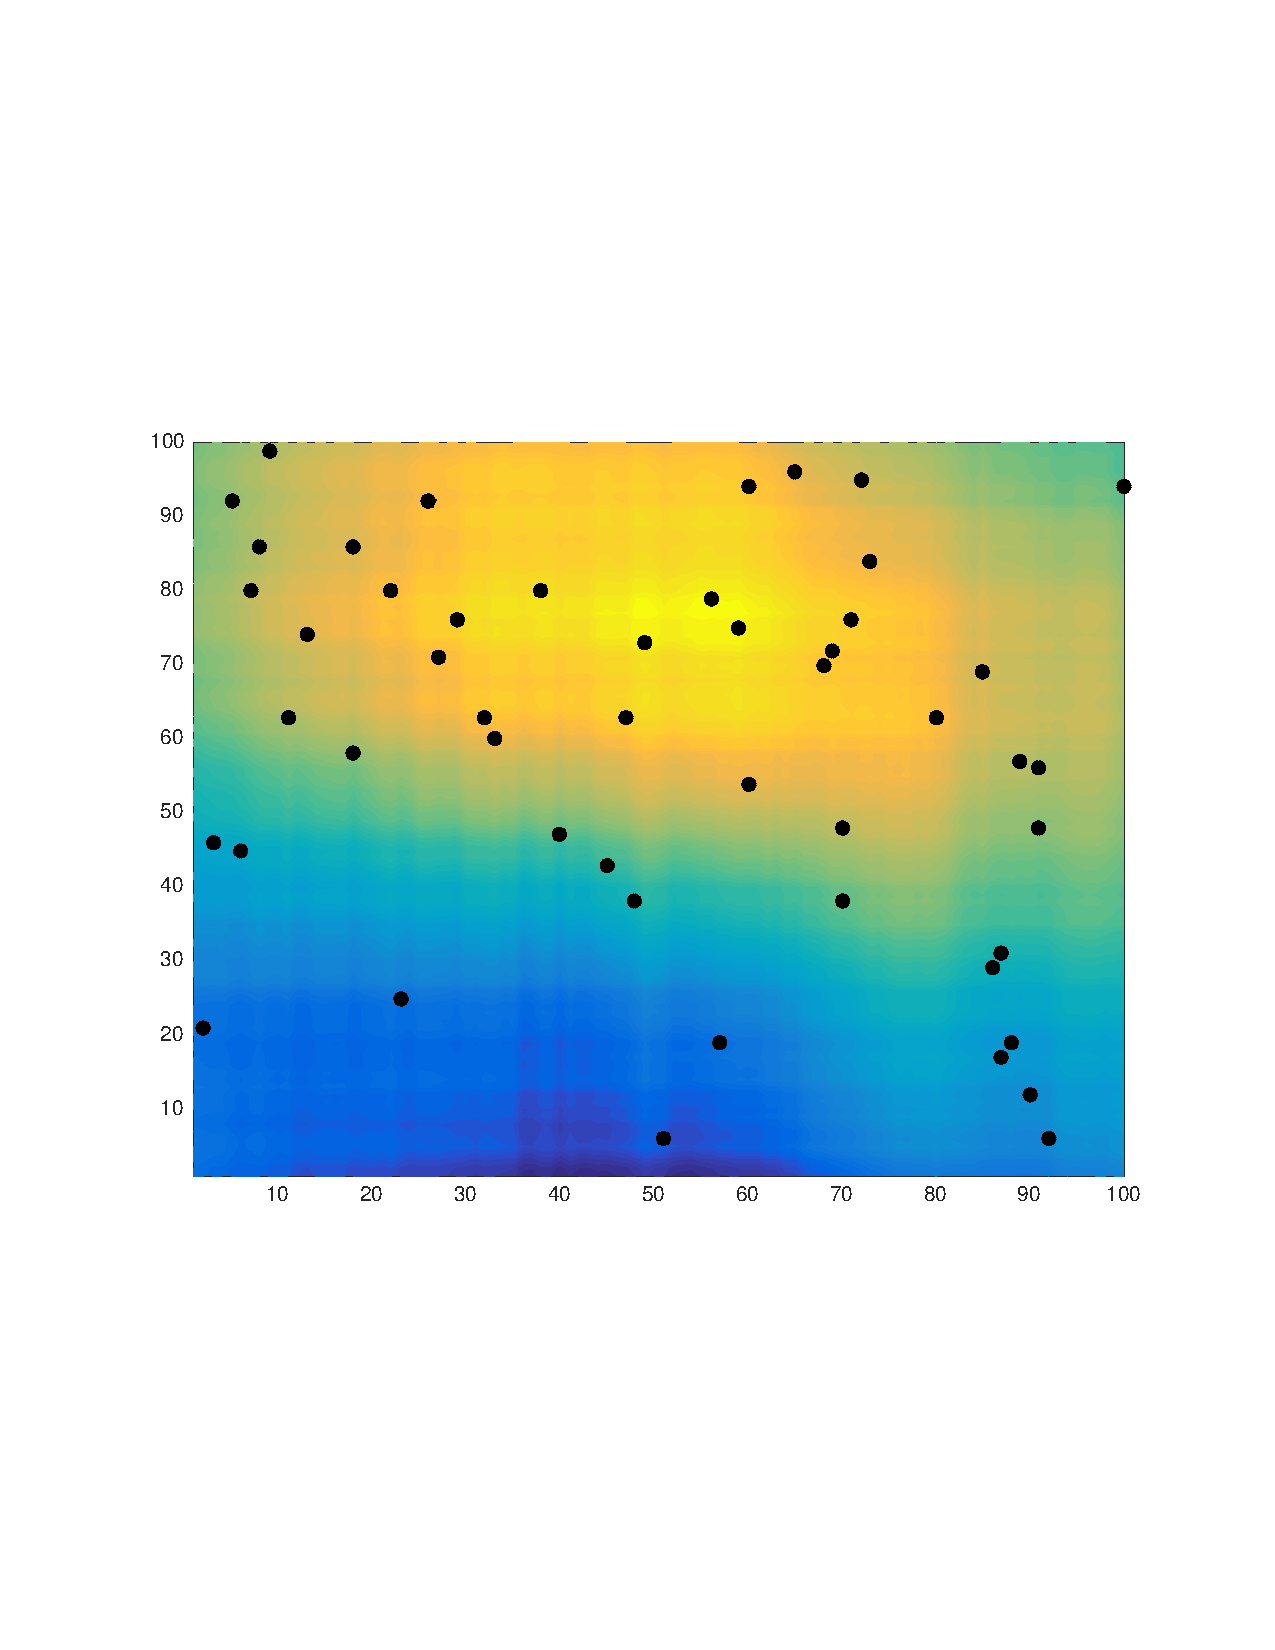
\includegraphics[width=\linewidth]{figures/sampled_generated_field.png}
		\captionsetup{skip=0.5\baselineskip,size=footnotesize}
		\caption{Samples at marked locations were taken of the target field in \ref{fig:gen_field}.}
		\label{fig:sampled_field}
    \end{subfigure}
    \caption{A Gaussian distributed randomly generated spatially autocorrelated field.}
    \label{fig:generated_and_sampled_field}
\end{figure}

\section{Inverse Distance Weighting} \label{sec:idw_intro}
An inverse distance weighting is a naive interpolation tool where a point is predicted based its distances from a set of observed points. A simple IDW, using Shepard's Method \cite{shepard:idw}, gives a prediction, $\hat{Z}(\vect{s}_j)$, of an unobserved point, $\vect{s}_j$, as a function of the $N \in \mathbb{N}$ observed points, $\{Z(\vect{s}_1), Z(\vect{s}_2), \hdots, Z(\vect{s}_n) \}$.

\begin{equation}
	\hat{Z}(\vect{s}_j)=\begin{cases}
			\dfrac{\sum\limits_{i=1}^N [w(\vect{s}_j, \vect{s}_i)] Z(\vect{s}_i) }{\sum\limits_{i=1}^{N} w(\vect{s}_j, \vect{s}_i)} & \text{if}\ \forall i \mid d(\vect{s}_j,\vect{s}_i) \neq 0\ \\
			Z(\vect{s}_j) & \text{if}\ \exists i \mid d(\vect{s}_j,\vect{s}_i)=0\\
		\end{cases}
\end{equation}
\begin{equation}
	w(\vect{s}_j, \vect{s}_i)=\frac{1}{d(\vect{s}_j,\vect{s}_{i})^{p}}=\|\vect{s}_j-\vect{s}_i\|_{2}^{-p}
\end{equation}

where $p \in \mathbb{R}^{+}$ is the IDW "power parameter". The power parameter, $p$, controls the emphasis on near and far observations on a prediction. As $p$ increases, the predicted values more closely resemble the closest made observation to the prediction location. Inversely, as $p$ gets smaller within $(0, 1]$, more emphasis is drawn from observations made further away.\\

\begin{figure}[ht!]
    \centering
    \includegraphics[width=0.8\linewidth]{figures/idw_predicted_field.png}
    \caption{An inverse distance weighting predicted field generated from the samples taken of Figure \ref{fig:gen_field} at the locations marked in Figure \ref{fig:sampled_field}.}
    \label{fig:idw_field}
\end{figure}

This method can yield a prediction for all possible $\vect{s}_j$ points in a field where a set of observations at known locations are made, as done in Figure \ref{fig:idw_field}. Unfortunately, the method is limited in that it does not take advantage of the underlying stochastic model, and spatial pattern, of the field, $Z$, being observed to make a more methodical weighted sum prediction. A more statistical approach will be introduced in Section \ref{sec:vario} on Variography to \textit{learn} the underlying statistical pattern and autocorrelation of a field.

\section{Variography} \label{sec:vario}
Variography is a set of procedures for examining and interpreting spatial dependence and geospatial autocorrelation in a field of observed data. In order to make a more intelligent weighted sum for a prediction, extracting the underlying geospatial autocorrelation function, the \textit{variogram}, of a field will be introduced. The variogram function will be factored into a classical prediction via weighting, yielding a Kriging Weighting.

\subsection{The Variogram}
A variogram quantifies dependence for two disjoint observations separated by some distance, or \textit{lag}, away. The function, in essence, yields a value directly proportional to the covariance between two given points in a stochastic field.

A Variogram is intended to be a continuous function which yields a covariance between two points $Z(\vect{s}_{i})$, $Z(\vect{s}_{j})$, which have not necessarily been observed, but known to be a Euclidean distance, or lag, $h_{i,j} \in \mathbb{R}$ apart, where

\begin{equation}
h_{i,j} = \| \vect{s}_i - \vect{s}_j \|_2
\label{eq:hdist}
\end{equation}

Using the assumption on what a point's value on a field is constructed of is made in Equation 2.4.1 of Matheron, 1963 \cite{matheron:geostat}:

\begin{equation}
    Z(\vect{s}_i)=\mu(\vect{s}_i)+\theta(\vect{s}_i)
    \label{eq:matheron:assum}
\end{equation}

Where $\theta(\cdot)$ is a zero-mean intrinsically stationary stochastic Wiener process. An assumption that the mean $\mu(\cdot) = \bar{Z}$ is only constant in a reasonably small neighborhood of $Z$. This becomes relevant when the sample sizes of the field increase where more reliable means will be derived from local neighborhoods. The size of the local neighborhoods to consider a constant field mean within will later be defined to be a function of the maximum autocorrelation lag, but no cut-off is required by definition.

\subsection{The Semivariogram}
The Semivariogram is defined to be the average squared difference between two points separated by some distance apart. Matheron, 1963 formally defines a variogram in \cite{matheron:geostat} in three-dimensional space. Using the notation used in this paper for a two-dimensional field, the Semivariogram will be defined as:

\begin{equation}
    \gamma(h) = \frac{1}{2A} \iint_A [ Z(\vect{s} + h) - Z(\vect{s}) ]^2 dA
    \label{eq:semivariogramint}
\end{equation}

Where $A$ is a closed area in a field, $Z$, to consider, $Z(\vect{s})$ is the value of a point at location $\vect{s}$ on the field $Z$, and $Z(\vect{s} + h)$ is the value of some point a distance $h$, defined in Equation \ref{eq:hdist}, apart from a point $\vect{s}$ on the field $Z$.

It is infeasible to estimate an observation value at each possible point in the field to compute a continuous Semivariogram. Furthermore, the fields observed using these methods are typically gridded, and therefore not continuous by their analytical nature. A discrete model must first be constructed, and will then be fit into a continuous variogram model. This is done by first constructing a discrete variogram model, or \textit{Empirical Semivariogram}, and then fitting a continuous model to it. Fitting a discrete Semivariogram should in turn yield a function close to $\gamma(h)$ defined in Equation \ref{eq:semivariogramint}, and should be identical given that every point in the area $A$ is sampled with infinite precision.

\subsection{The Empirical Semivariogram}
An Empirical Semivariogram, or Experimental Variogram, is a discrete function representing the covariance of the observation value difference between two sampled locations that are some distance $h$ apart. By modifying equation 2.4.2, Matheron, 1963 \cite{matheron:geostat} to include an additional boundary to classify a "bin", for two observations $\vect{s}_{i}$ and $\vect{s}_{j}$ in a stochastic field, $Z$, the experimental semi-variogram is defined to be:

\begin{equation} 
    \label{eq:exp_var}
    2\hat{\gamma}(h) := \frac{1}{|N(h,\delta)|}\sum\limits_{\forall \vect{s}_i,\vect{s}_j \in N(h, \delta)}|Z(\vect{s}_i) - Z(\vect{s}_j)|^2 % (Cressie 1993)
\end{equation}

Where $N(h,\delta)$ is the set of all pairs of observed points that are a distance in the interval $[h-\delta, h+\delta]$ away. This distance is referred to as the \textit{lag} between two points. If $\delta = 0$, the semi-variogram is not said to be \textit{binned}.

The experimental variogram conveys the geospatial autocorrelation of a sampled field. As the lag between two given points increases, the covariance also increases. The covariance levels out to a steady value (the \textit{sill}) at some distance in the domain (the \textit{range}). This position in the function marks where the loss of reliable geospatial autocorrelation between two points that are a distance $h$ apart lays.

\subsection{Converting a Semivariogram to a Variogram} \label{sec:semitovar}
The intent of fitting a statistical model to an experimental variogram is to approximate the continuous covariance for any two points, that have not necessarily been observed, on $Z$ that are at some known lag apart.

\subsection{Variogram Models} \label{sec:variomodels}
The Empirical Semivariogram will be fit to a statistical model, or \textit{kernel}, known as a Variogram Model. There exist some well known models, further discussed in this section. Each model is a scalar function of lag, $h$, \text{sill}, $s$, and \text{range}, $a$. The term \textit{sill} refers to the point on the codomain where two points at the lag specified are no longer autocorrelated. The sill is therefore the largest value of covariance for two disjoint points on a field that are still considered to be autocorrelated. The corresponding point on the domain for the sill is referred to as the \textit{range} on the variogram. Two points that have a lag larger than the range are not considered to be autocorrelated.

The \textit{nugget} of the variogram is defined to be the variance at zero separation, or $\gamma(0)$. This value is exactly zero for ideal measurements, but is generally not for real-life measurements. The value found for the nugget is typically summed with the value yielded by $\gamma$, to get the final covariance for a given lag.

\subsubsection{The Gaussian Model}

\begin{equation}
	\gamma_g(h, s, a) = s \Bigg[ 1 - \exp \Bigg( -\dfrac{h^2}{a^2} \Bigg) \Bigg]
	\label{eq:gauss_model}
\end{equation}

The Gaussian model will asymptotically reach its sill. The sill would be at the limit as $h$ approaches infinity. The \textit{practical range} is therefore used to refer the point on the domain where the variogram reaches 95\% of its sill.

\subsubsection{The Exponential Model}

\begin{equation}
	\gamma_e(h, s, a) = s \Bigg[ 1 - \exp \Bigg( \dfrac{h}{a} \Bigg) \Bigg]
	\label{eq:exp_model}
\end{equation}

The same rules as the Gaussian model apply to the Exponential model.

\subsubsection{The Spherical Model}

\begin{equation}
	\gamma_s(h, s, a) = \frac{s}{2} \Bigg[ \dfrac{3h}{a} - \Bigg( \dfrac{h}{a} \Bigg)^3 \Bigg]
	\label{eq:sph_model}
\end{equation}

The spherical model will reach an exactly zero slope at the sill and range.

\subsection{Fitting A Semi-Variogram} \label{sec:varfit}
The kernel function of the range, $a$, the sill, $s$, and lag, $h$ is chosen based on the statistical properties of the field being examined. For example, a field that is known to have normally distributed stochastic values, should be predicted using a Gaussian Model. The model chosen could then be used as the objective function in a numerical nonlinear multivariate solver, for example, to find the appropriate values for $a$ and $s$. Once $a$ and $s$ are found, the model can be used to yield the covariance between two points on the field a distance $h$ apart. Furthermore, as more samples of the target field are taken, the values found for $a$ and $s$ better depict the spatial statistics of the field.

\subsubsection{Fitting a Variogram Using MATLAB}
Using a version of the \textit{fminsearch} function in \textit{MATLAB}, a variogram can be fit to the desired objective function from a set of samples, and initial guesses for the range and sill. As the function is used over several iterations of sampling, the fit range and sill values found in the previous iteration can be used as the seed to the next iteration of the fit in an attempt to minimize computation time. The function is defined to ``find the minimum of an unconstrained multi-variable function using a derivative-free method", expressed in Equation \ref{eq:matlabfmin}.

\begin{equation}
\gamma(h) = \min\ [\gamma_{kernel}(h,s,a) - \hat{\gamma}(h)]^2
\label{eq:matlabfmin}
\end{equation}

The function is then modified by specifying bounds of minimization in an attempt to decrease iterations of the function fit, which can be computationally expensive as more samples are taken. This modified version of \textit{fminsearch}, named \textit{fminsearchcon}, can be downloaded from the MathWorks File Exchange.

\begin{figure}[ht!]
    \centering    
	\includegraphics[width=\linewidth]{figures/fit_kernel.png}
	\caption{An experimental variogram generated using Equation \ref{eq:exp_var} from the samples taken in Figure \ref{fig:sampled_field}. $\delta$ was chosen such that for $n$ observations, a total number of $\Big\lfloor \frac{n}{2} \Big\rfloor$ points were plotted. A Gaussian statistical model was fit to the experimental variogram. The variogram was fit using \textit{fminsearchcon} in \textit{MATLAB}.}
	\label{fig:fit_kernel}
\end{figure}

\section{The Kriging Method}
The Kriging Method conducts a weighted sum using the continuous variogram model that was fit to the physical observations made. The method can yield a prediction for each vesicle in a target space similar to the Inverse Distance Weighting method described in Section \ref{sec:idw_intro}, but with more statistical robustness.

\subsection{Forms of the Kriging Method}
There exist three major forms of the Kriging Method. All of which differ primarily in the handling of the mean gathered from observations of a target field. The \textit{Simple Kriging Method} makes the assumption that the mean is known and constant throughout the entirety of an observed field. This is of course not the case for fields that are very large as it does not follow Tobler's First Law. The \textit{Ordinary Kriging Method} can deduce the local mean of a neighborhood from a smaller subset of observations in a larger target field. This is done by classifying the larger field into smaller neighborhoods where the mean is only constant within those neighborhoods. Ordinary Kriging has the advantage that the mean is not required to be known before running a prediction. The \textit{Universal Kriging Method} can perform similar local mean calculations as the Ordinary Kriging Method, but does so by fitting a polynomial representing a mean trend model and not from a constant mean value representing that neighborhood \cite{vandergraaf:nnkrig} as seen in Section \ref{sec:varfit} on fitting a variogram.

\subsection{Covariance Matrix From A Variogram} \label{sec:covmat}
From the fit variogram which represents our lag covariances, a \textit{covariance matrix} for $N$ observations, $P \in \mathbb{R}^{N \times N}$, will be constructed. The value of the element $P_{i,j}$, will represent the covariance of the lag between the $i^{th}$ and $j^{th}$ observations. If $i=j$, the value of the element, $P_{i,j}$ would be the variance of that observation. 

\begin{equation}
    P_{i,j} = \text{cov}\{Z(\vect{s}_{i}), Z(\vect{s}_{j})\} = \gamma(\| \vect{s}_i - \vect{s}_j \|_2)
    \label{eq:covvarmatelem}
\end{equation}

\begin{equation}
    P = \begin{bmatrix} 

    \text{var}\{\vect{s}_1\} & \text{cov}\{\vect{s}_1, \vect{s}_2\} & \dots & \text{cov}\{\vect{s}_1, \vect{s}_N\} \\
    
    \text{cov}\{\vect{s}_2, \vect{s}_1\} & \text{var}\{\vect{s}_2\} & \dots & \text{cov}\{\vect{s}_2, \vect{s}_N\} \\

    \vdots & \vdots & \ddots & \vdots  \\
    
    \text{cov}\{\vect{s}_N, \vect{s}_1\} & \text{cov}\{\vect{s}_N, \vect{s}_2\} & \dots & \text{var}\{\vect{s}_N\} \\

    \end{bmatrix}
    \label{eq:covvarmat}
\end{equation}

\subsection{The Proximity Vector} \label{sec:proxvect}
For any given point on a field, we can construct a \textit{proximity vector}, $\vect{d}_0 \in \mathbb{R}^N$, which contains the covariance of a given point, $\vect{s}_0$ on the field with the $N$ observations made. The $k^{th}$ element of $\vect{d}_N$, would therefore contain the covariance for the lag between point $\vect{s}_0$ and the $k^{th}$ observation made, $\vect{s}_k$.

$$\vect{d}_0(k) = \text{cov}\{Z(\vect{s}_0), Z(\vect{s}_k)\} = \gamma(\| \vect{s}_0 - \vect{s}_k \|_2)$$

\begin{equation}
    \vect{d}_0 = \begin{bmatrix} 
                    \text{cov}\{Z(\vect{s}_0), Z(\vect{s}_1)\} \\
                    \text{cov}\{Z(\vect{s}_0), Z(\vect{s}_2)\} \\
                     \vdots \\
                    \text{cov}\{Z(\vect{s}_0), Z(\vect{s}_N)\} \\
        \end{bmatrix} = 
        \begin{bmatrix} 
                    \gamma(\| \vect{s}_0 - \vect{s}_1 \|_2) \\
                    \gamma(\| \vect{s}_0 - \vect{s}_2 \|_2) \\
                     \vdots \\
                    \gamma(\| \vect{s}_0 - \vect{s}_N \|_2) \\
        \end{bmatrix} 
    \label{eq:proxvect}
\end{equation}

Furthermore, The Kriging Method can be \textit{bounded}. If a to-be-predicted point and a given sample is beyond the range value fit to the variogram model, the corresponding element in the proximity vector is set to the sill. This ensures that points outside of the range of autocorrelation are not weighted anymore than they should be. This method is suggested when the variogram model used is a \textit{bounded function}, e.g. the Spherical Model (Equation \ref{eq:sph_model}).

\subsection{The Kriging Weights} \label{sec:krigweights}
Similarly to the Inverse Distance Weighting method, a set a weights will be computed for each vesicle in the target field. These weights will be referred to as the \textit{Kriging Weights}, or the \textit{error variance vector}. For a given prediction location, $\vect{s}_0$, the Kriging Weight vector, $\vect{\lambda}_0$, will be defined as the product of the inverse of the covariance matrix of the field and the proximity vector of the point to predict.

\begin{equation}
    \vect{\lambda}_{0} = P^{-1}\vect{d}_{0}
    \label{eq:krigweights}
\end{equation}

\subsection{The Kriging Prediction Equation}
The Kriging equation will be used to predict the value, $\hat{Z}(\vect{s}_0)$ of an unobserved location, $\vect{s}_0$. The prediction is a function of the Kriging Weights and a vector of $N$ observations. 

\begin{equation}
    \hat{Z}(\vect{s}_0) = \begin{bmatrix} Z(\vect{s}_1) & Z(\vect{s}_2) & \dots & Z(\vect{s}_N) \end{bmatrix}\vect{\lambda}_{0}
    \label{eq:krigeq}
\end{equation}

\begin{figure}[!]
    \centering
    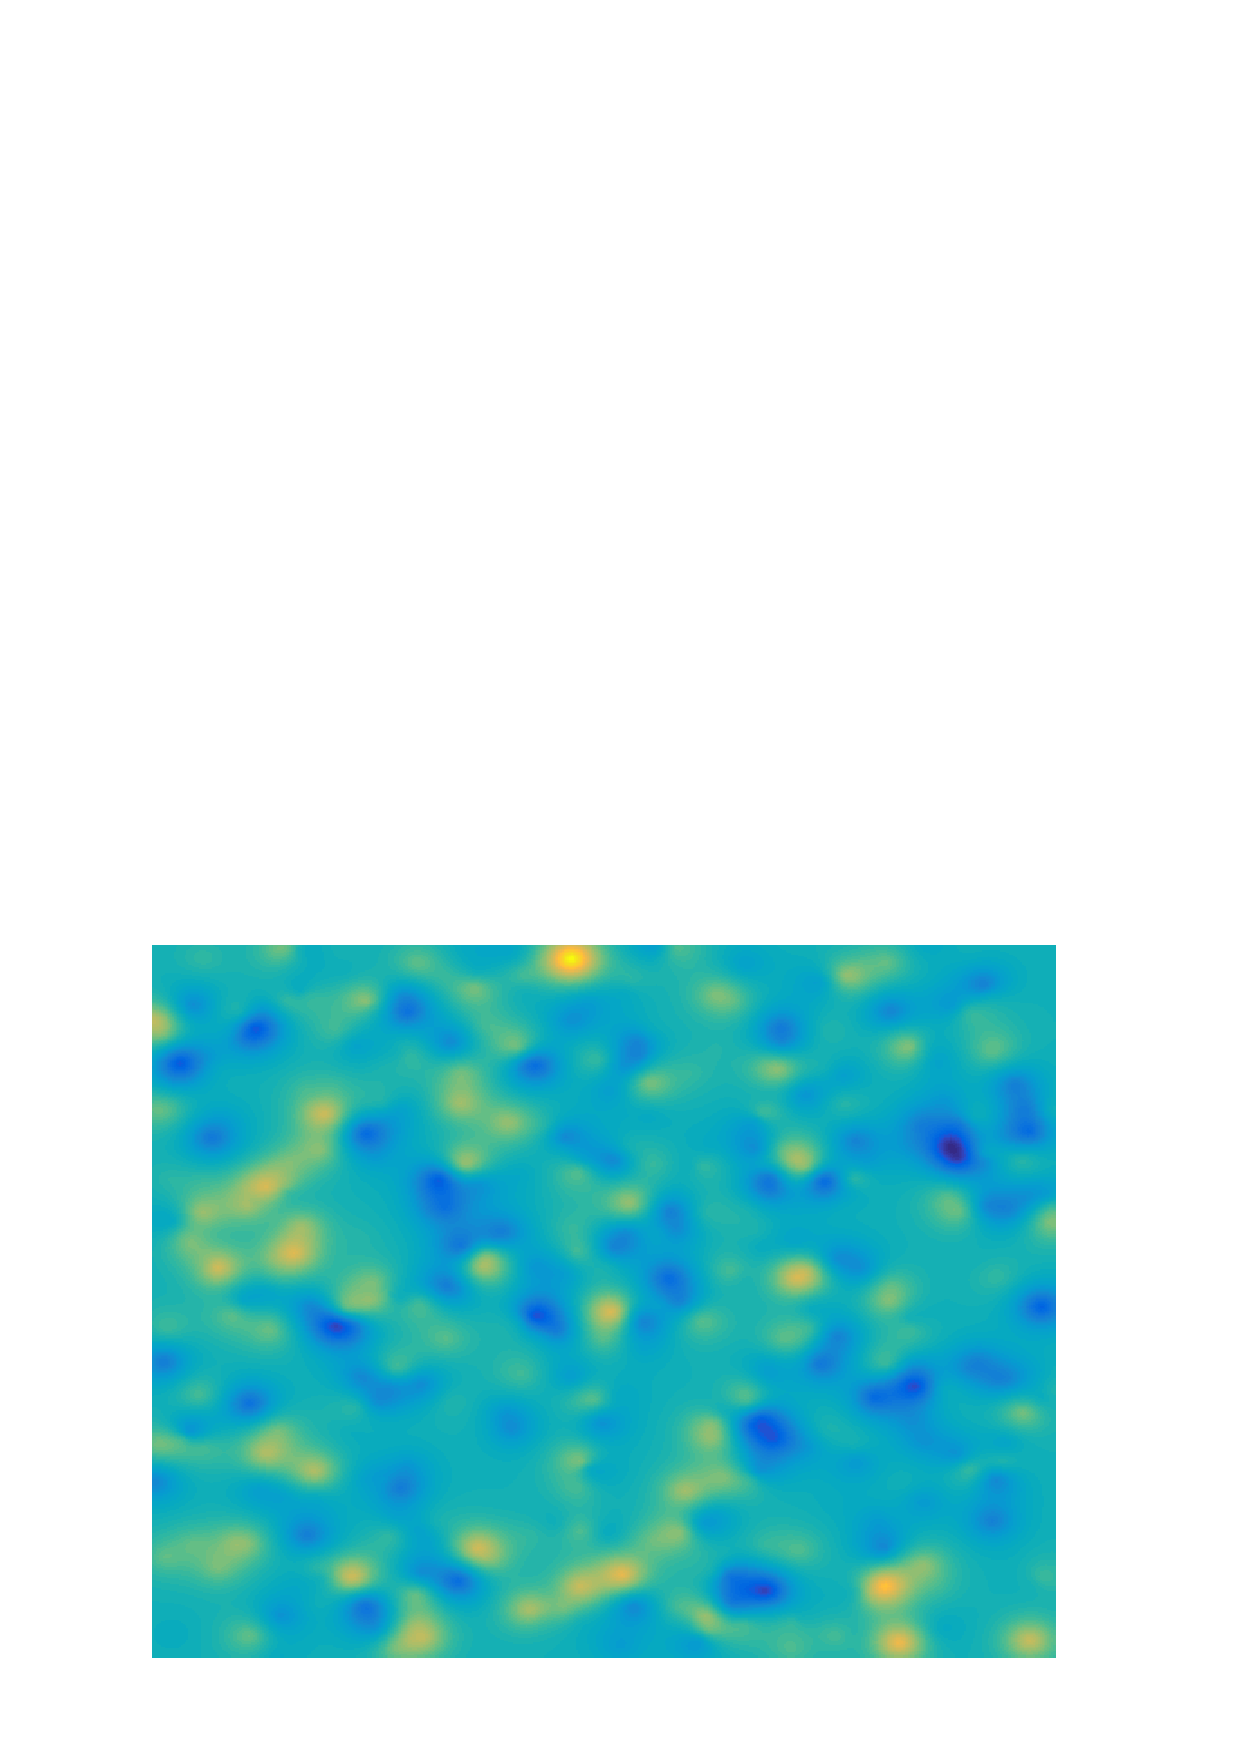
\includegraphics[width=0.8\linewidth]{figures/kriging_prediction.png}
    \caption{A Kriging Method predicted field generated from the samples taken of Figure \ref{fig:gen_field} at the locations marked in Figure \ref{fig:sampled_field}.}
    \label{fig:krig_field}
\end{figure}

\subsection{Variance of A Kriging Prediction}
The variance of a point predicted on a target field can be calculated using byproduct terms generated along the way of calculating a Kriging prediction. For a predicted point $\hat{Z}(\vect{s}_0)$, using the proximity vector, $\vect{d}_0$, defined in Section \ref{sec:proxvect}, and the Kriging Weights, $\vect{\lambda}_0$ defined in Section \ref{sec:krigweights} for the predicted point, the variance of the prediction for that point is defined as:

\begin{equation}
    \text{car}(\hat{Z}(\vect{s}_0)) = \vect{d}_0 \cdot \vect{\lambda}_0 = \vect{d}_0 \vect{\lambda}_0^T
\end{equation}

\subsection{The Kriging Error}
% look at the wikipedia page
From the method described in Equation \ref{eq:krigeq}, an error can be computed by comparing the predicted value of a previously observed point, $\hat{Z}(\vect{s}_p)$, to the observed value of the point, $Z(\vect{s}_p)$.

\begin{equation}
    \tilde{Z}(\vect{s}_p) = \hat{Z}(\vect{s}_p) - Z(\vect{s}_p) 
    \label{eq:krigerr}
\end{equation}

The Kriging Error value will be used to test the unbiasedness of the predictions made, and is factored into confidence of predictions made.

\subsection{Procedure For Field Prediction Using The Kriging Method}
In order to predict the entirety of a target field from a finite set of $N$ observations and their respective locations, $O$, the Kriging Prediction is run at every possible unobserved vesicle in the target field, $Z$. For a single iteration of collecting observations and making predictions, a covariance matrix must first be constructed, and then a the proximity vector and Kriging Weights are computed for all unobserved vesicles. The Kriging prediction formula is then used to compute the predicted value of each vesicle to predict.

\begin{algorithm}[thpb!]
\caption{Kriging Prediction of Target Field}\label{alg:krig}
\begin{algorithmic}[1]
\Procedure{KrigingPredictField}{$Z$, $O$}
\BState \emph{Generate Semi-Variogram}:
\State $\forall$ $\vect{s}_i$, $Z(\vect{s}_i)$ $\in O$:
\State \ \ \ \ $\hat{\gamma}(h) \gets \vect{s}_i$, $Z(\vect{s}_i)$\\
\BState \emph{Generate Variogram}:
\State $\gamma(h)$ fits to $\hat{\gamma}(h)$\\
\BState \emph{Construct Covariance Matrix}:
\State $\forall (\vect{s}_i,\vect{s}_j) \in O:$
\State \ \ \ \ $h_{i,j} = \|\vect{s}_i - \vect{s}_j\|_2$
\State \ \ \ \ $P_{i,j} = \gamma(h_{i,j})$\\
\BState \emph{Run Kriging Predictions For Target Field}:
\State $\forall$ $\vect{p}_i \in Z$:
\State \ \ \ \ $\vect{d}_{i} = \begin{bmatrix} \gamma(\| \vect{s}_1 - \vec{p}_i \|_2) \dots \gamma(\| \vect{s}_N - \vec{p}_i \|_2) \end{bmatrix}^T$
\State \ \ \ \ $\lambda_{i} = P^{-1}\vect{d}_{i}$
\State \ \ \ \ $\hat{Z}(\vect{p}_i) = \begin{bmatrix} Z(\vect{s}_1) \dots Z(\vect{s}_N) \end{bmatrix} \lambda_{\vec{p}_i}$
\EndProcedure
\end{algorithmic}
\end{algorithm}

When Algorithm \ref{alg:krig} is run on the target field from Figure \ref{fig:gen_field}, for the samples taken in Figure \ref{fig:sampled_field}, a prediction of the entire field can be generated, as seen in Figure \ref{fig:krig_field}.

% \part{Autonomous Field Exploration Using The Kriging Method}
\chapter{Path Planning} \label{ch:pp}
The goal of each of the planners introduced is to assist in the discovery of a field's features with an adjustable trade off between speed and confidence of prediction. The user of such a system could choose to scan more area if fuel is not of high concern. Likewise, if the field is very large, or several fields need to be scanned in a limited amount of time, a quicker scan with a lower degree of prediction certainty can be performed.

\section{Field Uncertainty Model} \label{sec:fielduncert}
The hypothesis that intentionally suppressing prediction variance yields a higher quality field prediction is used as the basis of the path planners introduced. The root mean square (RMS) error of any estimator is composed of two parts: a bias and variance of the estimate about the bias. The RMS error is reduced by reducing the variance of estimates. A Best Linear Unbiased Prediction method, such as the Kriging method, can therefore produce higher quality estimates with lower prediction variances.

A method for calculating the variance of a prediction was defined as a function of the proximity vector and Kriging weights generated for the prediction point in Equation \ref{eq:krigvar}. For points that have been directly measured, the variance is ideally zero (for fields with no drift or dynamics). The uncertainty of the prediction of a point in the target field is the variance of its prediction. The goal of a path planner intending to suppress uncertainty of all predictions in a target field would be to reduce the overall variance of the target field being explored.

Let $\Sigma(\cdot)$ be a criterion for overall predicted field uncertainty. The function can be defined as the average variance calculated from a prediction of all $h\times w$ predictable points on a target field from a set of observations, $S$.

\begin{equation}
	\Sigma(\hat{Z}_{S}) = \frac{1}{hw}\sum_{i = 1}^{hw} \text{var}\{\hat{Z}_{S}(\vect{p}_i)\}
	\label{eq:fielduncert}
\end{equation}

\noindent where $\Sigma(\hat{Z}_{S}) \in \mathbb{R}_{\geq 0}$ and $\text{var}\{\hat{Z}_{S}(\vect{p}_i)\} \in \mathbb{R}_{\geq 0}$ is the variance of the prediction of the $i^{th}$ point, $\vect{p}_i$, when the field is predicted from a set of samples, $S$.

\subsection{Uncertainty Loss Function} \label{sec:lossfunc}
A criterion for overall field uncertainty was introduced in Section \ref{sec:fielduncert}. Given a set of sampled points, $S$ on a field, the overall field uncertainty is the mean variance of all points on the field, $\Sigma(\hat{Z}_{S})$. For an additional set of samples, $T$, taken on the field, a new field uncertainty, $\Sigma(\hat{Z}_{S \cup T})$, is the field uncertainty criterion of the fields prediction from the union of the sample sets $S$ and $T$. The difference in overall field uncertainty, $L(T)$, will be defined as the uncertainty lost by taking the additional samples in the set $T$ on the field.

\begin{equation}
	L(T) = \Sigma(\hat{Z}_{S}) - \Sigma(\hat{Z}_{S \cup T})
	\label{eq:lossfunc}
\end{equation}

% The optimal path, $O$, subject to a limited scanning time constraint, is the path that simultaneously maximizes $L(S,O)$, and minimizes the length of of the path taken (using the assumption of a constant linear velocity from Section \ref{sec:vehicledynamics}).

% \begin{equation}
% 	O = \argmax_T\ \beta L(T) - (1-\beta)l(S + T)
% \end{equation}

% \noindent where $\beta \in [0,1]$ is a real number which puts more emphasis on exploration time over prediction quality. It is important to note that as more samples are taken, the overall field prediction variances change. It would be in the benefit of a path planner to batch process a set of points after meeting a predetermined waypoint, or after a threshold number of samples. 

% Given an endpoint in a single trajectory, in the limit, recalculating $O$ at every sample would optimally shape the trajectory of the exploration vehicle. With no endpoint selected, the exploration vehicle could be found in a repeating state due to being stuck in a global minimum in the variance field. In an effort to avoid the sticking minimum problem, the path planners introduced will be endpoint oriented (where the endpoint of any trajectory is predetermined), and the goal of each path taken is to make it to the endpoint. Furthermore, a new path will only be calculated as a batch process after sampling a trajectory. This is done in an attempt to reduce computation time as the Kriging predictions and variance calculations become more expensive as more samples are taken.

% \section{Finding Points of Highest Uncertainty} \label{sec:highestvars}
% Points on a target field with high prediction uncertainties should be sampled in order to reduce overall field uncertainty. After sampling an initial set of points, and then running a Kriging prediction on all points on a target, the variance of prediction of all points can be calculated.

% The motivation of the path finders introduced is to minimize the average uncertainty of a target field by sampling the points representing the highest prediction variances on the field. A set of points where the highest uncertainties lie are found on the field using a simple search.

% Let $S_k$ be a singleton set containing the point of highest variance on the $k^{th}$ iteration of the target field prediction variances, represented as the set $\text{var}\{\hat{Z}_k\}$, where $\text{var}\{\hat{Z}\} : \mathbb{R}^2 \to \mathbb{R}^+$.

% \begin{equation}
% 	S_{k} = \argmax_{\vect{s}} \ \text{var}\{\hat{Z}_{k}(\vect{s})\}
% 	\label{eq:highestvar}
% \end{equation}

% \noindent The cardinality of the set $S_k$ can be greater than one if there exist multiple instances of the same value of variance in the target field prediction variances. For the sake of simplicity, only the singleton case will be considered.

% Let $\text{var}\{\hat{Z}_{k+1}\}$ be the set of points, not including the point of highest variance found in the $k^{th}$ iteration of the set configuration (Equation \ref{eq:highestvar}), on a target field prediction.

% \begin{equation}
% 	\text{var}\{\hat{Z}_{k+1}(\vect{s})\} = \text{var}\{\hat{Z}_k(\vect{s})\} - S_k \\
% 	\label{eq:nextmaxvarsset}
% \end{equation}

% \noindent Let $S_{v}$ be the set of the $N$ points of highest uncertainty on the target field prediction variances, $\text{var}\{\hat{Z}\}$.

% \begin{equation}
% 	\label{eq:highestvarsunion}
% 	S_{v} = \bigcup_{k = 1}^{N} S_k = \bigcup_{k = 1}^{N} \text{var}\{\hat{Z}_k(\vect{s})\} - \text{var}\{\hat{Z}_{k+1}(\vect{s})\}
% \end{equation}

\section{Path Planning Overview}
Five variance suppressing path planners are introduced in this thesis. Each of five path planners attempts to reduce Kriging prediction variance by steering an exploration vehicle through a target field in a fashion that is predicted to reduce overall field uncertainty. All five of the path planners introduced will need an initial set of samples to make an initial path decision. Each of the five path planners begin by conducting an initial sweep on the main diagonal of the field. They initially stop at a waypoint set to a point close to the middle point on the field. The first point is the point in which the zig-zag method (discussed in Section \ref{sec:zz}) initially stops. The initial set of samples taken from the sweep will then be used to make an initial decision.

\section{Highest Variance Path Planner} \label{sec:nhvpp}
The \textit{Highest Variance} (HV) Path Planner attempts to reduce field prediction uncertainty by setting the exploration vehicle's destination to the point of highest prediction variance on the field. After meeting the point of highest variance, the field prediction and variances are recalculated from the samples the vehicle took on its path to the previously selected destination point. The next destination, or \textit{decision point}, is then set to the new point of highest prediction uncertainty.

Sampling the location of the highest variance is the simplest and most naive approach to path planning using the Kriging method. The highest point of uncertainty on the field is the point, $\vect{p}$, is defined as:

\begin{equation}
\argmax_{\vect{p}} \ \text{var}\{\hat{Z}(\vect{p})\}
\end{equation}

By simply setting the next decision point of the path to $\vect{p}$, the point of highest uncertainty will be sampled at the end of the path. Once the point is met at the end of the path, a new set of samples gathered from the path to the endpoint will be used to recalculate the statistical patterns of the field to higher degree of quality. A Kriging prediction, variances of those predictions are then run on the field. The path planner continues by setting the next decision point to the point of highest uncertainty after recalculating the variances of the field. The planner terminates exploration once a preset maximum scan area limit has been met by the exploration vehicle.

\subsection{Inefficiency in Highest Variance Method}
The HV algorithm does not account for repeating paths, or avoiding the re-sampling of points on the field. The only knowledge used is the variance of the endpoint of a path. Although the ground covered by the algorithm may be sufficient for uncertainty suppression, a path planner that considers the cost of trajectories would likely yield better results.

\section{$N$ Highest Variances Path Planner} \label{sec:nnhv}
The \textit{$N$ Highest Variances} (N-HV) Path Planner sets its decision point to a point from a set of the $N$ points of highest prediction variances. A \textit{leg}, or trajectory between the current position of the exploration vehicle and a potential decision point is calculated for all points in the set. The leg that is predicted to reduce the most overall field uncertainty (Equation \ref{eq:fielduncert}) is set as the next decision point of the vehicle. When the decision point is met, the set of legs to the $N$ highest variances is recalculated. The next decision point is set to the point that yields the leg that is expected to maximize loss in field uncertainty.

Let $K_N$ be the set of the $N \in \mathbb{N}$ points of highest uncertainty on the field. Let $T_i$ be a candidate trajectory connecting the current position of the exploration vehicle to the $i^{th}$ point in the set $K_N$. The endpoint that is ultimately chosen by the $N$ Highest Variance Path Planner is the one that maximizes the loss function, $L(T_i)$. The points along a trajectory, $T_i$, have likely not been sampled, as they represent points of high uncertainty. The loss in uncertainty for taking the path, $T_i$, is therefore not known. An estimate of the loss in overall field uncertainty, $\hat{L}(T_i)$, after taking the path, $T_i$, is calculated by using the previous Kriging predictions of the points along the path. The predictions of those points are used as actual samples taken on the field in a new Kriging prediction variance calculation of the field.

\section{Monte Carlo Path Planner} \label{sec:mcpp}
The Monte Carlo Path Planner (MCPP) calculates a set of legs to the $N$ highest points of variance on the field, similarly to the $N$-HV planner, except that for each leg, a separate set of $M_{mc}$ random trajectories are calculated around the leg. The exploration vehicle trajectory, or set of waypoints to a decision point, that is selected, is the random trajectory that maximizes loss in field uncertainty. The samples taken along the last trajectory selected are stored and used to recompute field variances when the final point in the trajectory (decision point) is met. New possible trajectories are then recalculated, and the planner repeats until a predefined maximum exploration distance has been met by the vehicle. This method compares a total of $N M_{mc}$ noisy trajectories per decision point met. By introducing noise into each of the trajectories found in the $N$-HV path planner, a more optimal path may be found.

Let $K_N$ be the set of the $N$ points of highest prediction variances on the field. Let $T_i$ be a candidate trajectory from the current position of the exploration vehicle to the $i^{th}$ endpoint in the candidate endpoint set, $K_N$. Each point in the candidate trajectory is a waypoint the exploration vehicle will visit on its way to the last point in the sequence. The trajectory is a set of states representing the field position, $(x,y)$, and the vehicle heading angle, $theta$. The $k^{th}$ vector in the state candidate trajectory set, $T_i$, denoted as $T_{i}(k)$, will be the state the exploration vehicle will take on at that position on the field, i.e.

\begin{equation}
T_{i}(k) = \begin{bmatrix} x_i(k) \\ y_i(k) \\ \theta_i(k) \end{bmatrix}
\end{equation}

Let $\alpha \in \mathbb{R}$ be the step size of the vehicle from one point to the next within the trajectory, $T_i$. Let $\vect{w}_i \in \mathbb{R}^2$ be a vector of two zero-mean Wiener processes with a tunable process standard deviation which is less than the step size, $\alpha$. Furthermore, the step size of the vehicle, $\alpha$, can not be a value less than the distance the exploration vehicle can travel in one time-step.

\begin{equation}
\text{var}\{\vect{w}_i\} = \begin{bmatrix} \text{var}\{w_{i_x}\} \\ \text{var}\{w_{i_y}\} \end{bmatrix}
\end{equation}

\begin{equation}
\text{var}\{w_{i_x}\} < \alpha^2
\end{equation}

\begin{equation}
\text{var}\{w_{i_y}\} < \alpha^2
\end{equation}

The corresponding Monte Carlo path, or sequence of waypoints the exploration vehicle will make on its way to the candidate endpoint, $\vect{p}_i = [p_x\ p_y]^T$.

\begin{equation}
\label{eq:mcpp}
T_{i}(k) = \begin{cases}
	\begin{bmatrix}
		x_0 \\
		y_0\\
		\text{atan2}(p_y - y_0, p_x - x_0)
	\end{bmatrix} & : k = 1 \\

	\begin{bmatrix}
		\alpha \cos \theta_i(k) \\
		\alpha \sin \theta_i(k) \\
		\text{atan2}(p_y - y_i(k), p_x - x_i(k))
	\end{bmatrix} + \begin{bmatrix} 
		\vect{w}_i(k) \\
		0
	\end{bmatrix} & : 1 < k < \Big\lceil \frac{\|\vect{p} - \vect{s}\|_2}{\alpha} \Big\rceil \\


	\begin{bmatrix} p_x \\ p_y \\ 0\end{bmatrix} & : k = \Big\lceil \frac{\|\vect{p} - \vect{s}\|_2}{\alpha} \Big\rceil \\

\end{cases}
\end{equation}

\noindent where the initial point in the candidate trajectory is set to the current position, $\vect{s}=[x_0\ y_0]^T$ from the state vector of the exploration vehicle. Due to the uncertainty in length of the random trajectory generated, the number of waypoints in the candidate trajectory $T_i$ is fixed, such that $k \in [1, \Big\lceil \frac{\|\vect{p}- \vect{s}\|_2}{\alpha} \Big\rceil]$ (the number of points in the trajectory for a step size, $\alpha$, given zero variance noise added to the process). The last point in the candidate trajectory set is set to the corresponding endpoint from the set $K_N$.

\begin{figure}[hbt!]
	\centering
	\includegraphics[width=0.8\linewidth]{figures/brownian_motion_mc.png}
	\ssp
	\caption{Monte Carlo paths (black) surrounding deterministic $N$-HV paths (red). The starting point, ($\vect{s} = [50 \ 6]^T$), is indicated in green. The set $K_N$ contains $N=2$ endpoints ($K_N = [ 5 \ 80 ]^T, [ 95 \ 90]^T$). $M_{mc}=15$ random walks are generated for each endpoint. $\alpha=5$. The variance of the Wiener process states are $\frac{1}{2} \alpha$.}
\end{figure}

As introduced in the $N$-HV path planner, a candidate trajectory is generated for each of the candidate endpoints in the set, $K_N$. The candidate trajectory that maximizes the loss function, $L(T)$, is the path that is ultimately selected as the next vehicle trajectory. In an effort to find a more optimal trajectory, more than one random walk can be generated for each endpoint in the set $K_N$. The variable $M_{mc} \in \mathbb{N}$ will denote the number of random walks taken per endpoint in the set $K_N$.

% \begin{algorithm}[h!]
% \caption{Monte Carlo Path Planning (MCPP) with The Kriging Method}\label{alg:mcpp}
% \begin{algorithmic}[1]
% \Procedure{Kriging\_MCPP}{$Z$}
% 	\BState \emph{Conduct Initial Sweep}:
% 	\State SetWaypoint($[h\ w]^T$)
% 	\BState \emph{Krig The Field}:
% 	\State $\hat{Z}, \text{var}\{\hat{Z}\}$ = KrigingPredictField($Z$, $S$)

% 	\BState \textbf{while} $F > 0$ \textbf{and} $\Sigma_{\text{var}} > 0$:
% 	\State $P = []$
% 	\State $\Sigma_{\text{min}} = \infty$ \\

% 	\BState \ \ \ \ \emph{Find the highest field variances}:
% 	\State \ \ \ \ \textbf{for}\ $k = 1 \text{:} N$
% 	\State \ \ \ \  \ \ \ \ $S_{v}(k) = \argmax_{\vect{s}} \ \text{var}\{\hat{Z}_{k}(\vect{s})\}$
% 	\State \ \ \ \ \ \ \ \ $\text{var}\{\hat{Z}_{k+1}(\vect{s})\} = \text{var}\{\hat{Z}_{k}(\vect{s})\} - S_{v}(k)$\\

% 	\BState \ \ \ \  \emph{Calculate trajectories to all points found}:
% 	\State \ \ \ \  $\forall s_k \in S_{v}(k)$:
% 	\State \ \ \ \  \ \ \ \ $s_d = s_k$
% 	\State \ \ \ \  \ \ \ \ $f = \Big\lceil \frac{\|\vect{s}_c - \vect{s}_d\|_2}{\alpha} \Big\rceil$
% 	\State \ \ \ \  \ \ \ \ $T(1) = \begin{bmatrix} s_{c_x} \\ s_{c_y} \\ \text{arctan2}(s_{d_y} - s_{c_y}, s_{d_x} - s_{c_x}) \end{bmatrix}$
% 	\State \ \ \ \  \ \ \ \ $\forall i \in (1, f - 1)$:
% 	\State \ \ \ \  \ \ \ \  \ \ \ \ $T(i+1) = T(i) + \begin{bmatrix} \alpha \cos \theta(i) \\ \alpha \sin \theta(i) \\ \text{atan2}(s_{d_y} - T(i)_y, s_{d_x} - T(i)_x) \end{bmatrix} + \begin{bmatrix} \vect{w}(i) \\ 0 \end{bmatrix}$
% 	\State \ \ \ \  \ \ \ \ $T(f) = \begin{bmatrix} s_{d_x} \\ s_{d_y} \\ \theta_{f-1} \end{bmatrix}$\\

% 	\BState \ \ \ \  \ \ \ \  \emph{Calculate estimated field confidence for trajectory computed}:
% 	\State \ \ \ \  \ \ \ \  $\forall i \in [1, f]$:
% 	\State \ \ \ \  \ \ \ \  \ \ \ \ $\text{samples}(\hat{S}_T)$ += $\hat{Z}(T(i))$
% 	\State \ \ \ \  \ \ \ \  \ \ \ \ $\text{locations}(\hat{S}_T)$ += $T(i)$
% 	\State \ \ \ \  \ \ \ \  \ \ \ \ $\hat{Z}_T, \text{var}\{\hat{Z}\}_T$ = KrigingPredictField($Z$, $\hat{S}_T$)
% 	\State \ \ \ \  \ \ \ \  \ \ \ \ $\Sigma_{\text{var}}(T) = \text{avg}(\text{var}\{\hat{Z}\}_T)$\\

% 	\State \ \ \ \  \ \ \ \  \ \ \ \ \textbf{if} $\Sigma_{\text{var}}(T) < \Sigma_{\text{min}}$ \textbf{and} \text{length($T$)} $< F$:
% 	\State \ \ \ \  \ \ \ \  \ \ \ \ \ \ \ \ $\Sigma_{\text{min}} = \Sigma_{\text{var}}(T)$
% 	\State \ \ \ \  \ \ \ \  \ \ \ \ \ \ \ \ $P = T$\\

% 	\BState \ \ \ \  \emph{Navigate through the chosen path}:
% 	\State \ \ \ \  $\forall p \in P$:
% 	\State \ \ \ \  \ \ \ \ SetWaypoint($p$) 
% \EndProcedure
% \end{algorithmic}
% \end{algorithm}

% In Algorithm \ref{alg:mcpp}, the function \texttt{SetWaypoint()} is an abstracted function which steers the vehicle in the direction of the waypoint specified, and blocks the code instruction until the waypoint has been met. The function \texttt{length(}$T$\texttt{)} finds the arc length of the path by connecting all points in the trajectory, $T$. For a deterministically calculated trajectory, $T$, the arc length is $\alpha |T|$.

\section{The Gradient Ascent Path Planner}
The Gradient Ascent (GA) Path Planner reduces field prediction variance by maximizing the movement in the local variance field's gradient at every move. At every decision point, a circle, with radius $r \in \mathbb{R}_{\geq 0}$, is generated around the exploration vehicle. In order to approximate the field variance gradient surrounding the exploration vehicle, a small step size value for $r$ is chosen. In this thesis, $r=3$ vesicles is used. The point on the circle surrounding the exploration vehicle with the highest Kriging prediction variance is set as the next decision point.

\section{The Range Gradient Ascent Path Planner}
The Range Gradient Ascent (RGA) Path Planner is similar to the Gradient Ascent path planner, but it sets the radius of the candidate circle surrounding the exploration vehicle to the value of the range, $a$, on the field's variogram, i.e. ($r = a$). The points within the range circle are points that are considered spatially autocorrelated, and therefore predictable to a high degree of confidence. By navigating the exploration vehicle to a point on the edge of spatial autocorrelation, the vehicle is motivated to move to points of higher prediction variance as the planner continues to run.

\section{Other Planners}
The five planners introduced will be compared to two planners discussed in the Section \ref{sec:prev_works} on Previous Works. The first method, the zig-zag (ZZ) method, directs the exploration vehicle through a predetermined path which spirals through the entirety of the field. The second method, the Greedy Next-Best-View (NBV) \cite{fentanes:soilkrig}, attempts to reduce Kriging variance by redirecting an exploration vehicle to the point of highest prediction variance after each sample taken.

\subsection{Zig-Zag Method} \label{sec:zz}
A common approach to exploration and patrolling problems is the use of a zig-zag pattern. The methods introduced will be compared to a zig-zagging approach demonstrated in Nikhil Nigam, et al. \textit{Control and Design of Multiple Unmanned Air Vehicles for a Persistent Surveillance Task} (Part II.C.3, Figure 6, \cite{nigam:zigzag}). The method will run a Kriging prediction and variance calculation on the samples taken using the zig-zag explorer, even though a prediction is not specified in the original work. This is to generate measurable and comparable metrics against the path planners introduced.

The zig-zag exploration method will stop the field exploration process when the exploration vehicle traverses a predefined area to scan, $A_{scan}$. If the maximum scan area of a field is $w \times h$, and the percent of the field to scan is $p\%$, then the method will stop exploring when the area $A_{scan} = \frac{p}{100}wh$ of the field has been sampled. The spacing between each spiral bound, $r$, will be pre-calculated in an effort to allow the zig-zag method to cover as much of the field as possible.

\begin{equation}
	\label{eq:zigzagrad}
    r = \frac{100}{p}
\end{equation}

The zig-zag method starts at the first point on the field (upper-left corner), and moves to the waypoint coordinate ($\Large\lceil\frac{w}{2} - r \Large\rceil, \Large\lceil \frac{h}{2} - r \Large\rceil$). Every planner will set the initial waypoint of the exploration vehicle to this point on the field. This is done so the initial set of samples of each of the planners is identical.

\subsection{Greedy Next-Best-View}
The Greedy NBV method, demonstrated in \cite{fentanes:soilkrig}, triggers the selection of a new waypoint after every new sample is taken by the exploration vehicle. The point that is chosen is the point on the field with the highest Kriging prediction variance at the time of point selection. After the next sample is taken on the way to the point of highest variance, the planner recomputes the field's variogram model, Kriging prediction, and field variance to recalculate the next decision point. The Greedy NBV planner will initiate by conducting an initial sweep on the main diagonal of the field and stop at the middle point of the field. This is done in order to collect a set of samples to make an initial decision.

\section{Planner Discussion} \label{sec:discuss}
The Monte Carlo path planner takes into account a set of noisy trajectories, and compares their estimated return on investment similarly to the $N$-HV method. Given enough trajectories, as $N$ gets larger for $N$-HV and MCPP and $M_{mc}$ gets larger for MCPP, the planners could find a path that will reduce overall field uncertainty in a more brute-force way over the HV, GA, and RGA methods introduced. The disadvantages of MCPP and $N$-HV lie in the fact that the cost of each next move taken is not considered directly because an entire trajectory is considered, in its entirety, at once. A more optimal approach to this planner would be to take into consideration the cost of each waypoint selected on the trajectory, and amend only the best waypoints found along the way. Furthermore, the MCPP approach is more computationally expensive (for $N > 1$, $M_{mc} > 1$) when compared to HV and $N$-HV because of the need to re-predict the field for each candidate trajectory calculated. The GA method becomes more computationally expensive as more samples are taken on the field, as this makes it more difficult to recompute the variogram model and Kriging predictions for the field at each step of the path. The HV, GA, and RGA planners are the simplest to compute because they only require one run of the Kriging field predictions and variance calculations, followed by a simple search for the highest field variances from a specified set of points.

The Greedy Next-Best-View planner, though similar to the GA and RGA planners introduced, does not purposefully attempt to directly sample the point of highest prediction variance from a set of candidate points. Both the GA and RGA planners arrive at a point of high variance from a set of candidate points, and sample it, where as the Greedy NBV will only move in the direction of the point of highest variance. As the field sizes get larger, the point of highest variance could be relatively distant from the point that is actually explored using Greedy NBV. The Greedy NBV method is therefore not expected to do well for larger fields. This is because the exploration vehicle can run into the problem where it will stick in a low variance valley. Once trapped in the valley, the vehicle will repeatedly move between two previously explored points until the end condition is met. The method will only be compared to the introduced methods in this thesis using course as presented in \cite{fentanes:soilkrig}.

A preplanned method, like the zig-zag method, does not intentionally attempt to suppress overall field prediction uncertainty, and because of this, may not predict the states of interest of the field to a high enough degree of accuracy when compared to the direct variance suppression methods. The zig-zag method does however attempt to sample an even distribution of path across the target field, allowing the method to estimate the field states to a high degree of accuracy.

% \part{Simulation \& Results}
\chapter{Simulation Framework}
A simulation of the path planning algorithm was created to demonstrate the ability of the described method. The simulation includes a software in the loop vehicle with variable dynamics, a randomly generated variable autocorrelated field of variable size, and a path planning algorithm introduced in Algorithm \ref{alg:uncert}. The simulation also incorporates the ability to follow a preplanned route. The simulation will be used to demonstrate the abilities of the algorithm described, and comparisons to an algorithm with a preplanned trajectory. 

\section{UAV Model Dynamics}
The system dynamics of the UAV in the software in the loop simulation will be modeled after a Dubin's vehicle. This is done to demonstrate the versatility of the algorithm by using it on various vehicle types. The vehicle's system states will simply be the Cartesian coordinates, $[x_1\ x_2]$, of its position above the target field described in Section \ref{sec:sensor_measurements}. The third dimension of altitude above the field does not concern the path planning algorithm and will be omitted from the state vector. The heading angle, with respect to the positive $x_1$ axis, will be referred to as, $\theta$.

\begin{equation}
\label{equ:state_vector}
\vect{X} = \begin{bmatrix} 
			x_1 \\
			x_2 \\
			\theta
			\end{bmatrix}
\end{equation}

For a constant velocity of $v$, from Dubin's vehicle, the state configuration transition equation is given by Equation \ref{equ:state_prop}.

\begin{equation}
\label{equ:state_prop}
\dot{\vect{X}} = \begin{bmatrix} 
			v \cos\theta \\
			v \sin\theta \\
			\dot{\theta}
			\end{bmatrix}
\end{equation}

The system is ideally fully observable. The velocity, $v$, can be set at will in the software in the loop implementation. A real world implementation of the algorithm would cap $v$ to the maximum possible velocity the vehicle can travel at, or the maximum speed the vehicle can sample a vesicle on the target field at.

\section{Simulating a Geospatially Autocorrelated Field}
The target field in the simulation is generated from a normal distribution of a predefined expected value and variance. A Gaussian low-pass filter, with a preset value for its standard deviation, is then convolved with the normal randomly generated field to remove any \textit{high frequency} trends in the data. The result is a geospatially autocorrelated field, where similar features near each other blend together.

\chapter{Results}
The three path planners (NHV, N-NHV, and MCPP) introduced in Chapter \ref{ch:pp} all aim to reduce the overall prediction uncertainty of a field given a limited amount of flight time. They accomplish the task by calculating variances of a target field's predictions and attempting to choose a trajectory that reduces overall uncertainty. 

\section{Comparing The Method}
A common approach to exploration and patrolling problems is the use of a spiral, zig-zag, or lawn mower pattern. The methods introduced will be compared to equally time limited version of a zig-zagging approaches seen in Nikhil Nigam, et al. Control and Design of Multiple Unmanned Air Vehicles for a Persistent Surveillance Task (Part II.C.3, Figure 6, \cite{nigam:zigzag}). The method, for the sake of fairer comparison, will run a Kriging prediction and variance calculation on the samples taken using the zig-zag explorer. This is to generate measurable and comparable metrics against the path planners introduced. The path planners introduced will be compared against the zig-zag exploration method shown in Figure \ref{fig:zigzag4}.

\begin{figure}[hbt!]
	\centering
	\includegraphics[width=0.9\linewidth]{figures/zigzag_4panel.png}
	\captionsetup{skip=0.20\baselineskip,size=footnotesize}
	\caption{Zig-Zag exploration method with a line spacing of $r = 8$ units. A Kriging prediction and variance calculation is computed after completing the maneuver. The actual field that is being explored is shown in the upper left. The current prediction of the actual field is shown in the upper right. The variance of the current prediction of the field is shown in the lower left. The trace of the exploration vehicle's path taken to the point of termination (in red) is shown in the lower right panel. All distance units are in meters.}
	\label{fig:zigzag4}
\end{figure}

\subsection{Prediction Error Calculation}
The quality of each path planner will be judged by its ability to explore a field in a fixed amount of time. The prediction error of each method will be used as a metric of path planning quality. The actual values of the fields scanned are known in simulation, and for each rerouting iteration, the predictions and prediction errors will be recalculated.

The prediction error value for each field prediction made will be the mean of every vesicles root mean square (RMS) error (element by element).

\subsection{Variance Drop Calculation}
The variance of every target field over each iteration will be the average prediction variance of the field after every prediction recalculation. This criteria is introduced in Section \ref{sec:fielduncert} on field uncertainty. This metric relates prediction quality of the path planner to its predicted prediction quality. A drop in variance over iterations should signal a better prediction of the target field over that iteration, and less overall uncertainty of the target field.

\subsection{Simulation Results}
% The effectiveness of the method introduced varies based on the area of the target field being explored. For small fields, a naive zig-zag exploration may be more efficient and less computationally expensive. By modulating the dimensions of the target field, a comparison can be drawn demonstrating the effectiveness of the method versus a naive zig-zag approach.
The methods introduced will be compared to one another and the zig-zag method in terms of variance drop and prediction error on a set of $5$ randomly generated geospatially autocorrelated fields with $20\times20$ vesicles for a variety of area coverage limits.



\begin{equation}
	r = \frac{A_{scan}}{2}
\end{equation}

Where $A_{scan}$ is the maximum area to scan. For a maximum fraction of the field to scan, $c_max$, $A_{scan} = wc_{max}$.

\begin{table}[ht!]
\centering
	\begin{tabular}{ |p{3cm}||p{1cm}|p{1cm}|p{1cm}|p{1cm}|p{1cm}|  }
		\hline
		\multicolumn{6}{|c|}{$20 \times 20$ Size Final Field Prediction Error} \\
		\hline
		Coverage Limit ($A_{scan}$) & 20\% & 30\% & 40\% & 50\% & 75\% \\
		\hline
		Zig-Zag        & 5.1672 & 4.2207 & 4.0158 & 2.3060 & 4.8467 \\
		NHV            & 3.8790 & 4.2592 & 3.8460 & 2.1858 & 2.5332 \\
		N-NHV ($N=5$)  & 3.8845 & 4.2072 & 3.8900 & 2.1765 & 2.5253 \\
		MCPP  ($N=1$)  & 3.7645 & 4.2576 & 3.9061 & 2.1888 & 2.5485 \\
		\hline
	\end{tabular}
	\caption{Comparing field prediction errors for varying coverage limitations on a $20 \times 20$ size field. For the MCPP method runs, $20$ random paths were calculated for each trajectory.}
    \label{tab:20fieldprederr}
\end{table}

\begin{figure}[hb!]
	\centering
	\includegraphics[width=0.8\linewidth]{figures/pred_error_20x20_50percent_5runs.png}
    \captionsetup{skip=0.20\baselineskip,size=footnotesize}
	\caption{Normalized prediction error drops per replanning iteration averaged over exploring 5 randomly generated target fields of size $20 \times 20$ at a $50\%$ scan. The predictions for the zig-zag method are recalculated at every turn.}
\end{figure}

\begin{table}[ht!]
\centering
	\begin{tabular}{ |p{3cm}||p{1cm}|p{1cm}|p{1cm}|p{1cm}|p{1cm}|  }
		\hline
		\multicolumn{6}{|c|}{$20 \times 20$ Size Final Field Prediction Variance} \\
		\hline
		Coverage Limit & 20\% & 30\% & 40\% & 50\% & 75\% \\
		\hline
		Zig-Zag        & 3.2313 & 1.2784 & 1.6893 & 1.5046 & 4.4644 \\
		NHV            & 1.0212 & 0.8993 & 0.9472 & 0.3822 & 0.3381 \\
		N-NHV          & 1.4860 & 0.9438 & 0.9027 & 0.3819 & 0.3398 \\
		MCPP           & 1.2532 & 0.7021 & 0.6659 & 0.3238 & 0.2041 \\
		\hline
	\end{tabular}
	\caption{Comparing field prediction errors for varying coverage limitations on a $20 \times 20$ size field.}
    \label{tab:20fieldvar}
\end{table}

\begin{figure}[hb!]
	\centering
	\includegraphics[width=0.8\linewidth]{figures/vars_semilogy_20x20_50percent_5runs.png}
    \captionsetup{skip=0.20\baselineskip,size=footnotesize}
	\caption{Normalized semi-logarithmic variance drops per replanning iteration averaged over exploring 5 randomly generated target fields of size $20 \times 20$ at a $50\%$ scan. The variance for the zig-zag method are recalculated at every turn.}
\end{figure}

% \subsubsection{$50 \times 50$ Target Field Size}
% The methods introduced will be compared to one another and the zig-zag method in terms of variance drop and prediction error on a set of $5$ randomly generated geospatially autocorrelated fields with $50\times 50$ vesicles.

% % \begin{table}[htb!]
% % \centering
% % 	\begin{tabular}{ |p{3cm}||p{1cm}|p{1cm}|p{1cm}|p{1cm}|  }
% % 		\hline
% % 		\multicolumn{6}{|c|}{$50 \times 50$ Size Final Field Prediction Error} \\
% % 		\hline
% % 		Coverage Limit & 10\% & 20\% & 50\% & 75\% \\
% % 		\hline
% % 		Zig-Zag        & 1.2624 & 1.2236 & .. & .. \\
% % 		NHV            & 1.2932 & 1.2228 & .. & .. \\
% % 		N-NHV          & 1.2932 & 1.2214 & .. & .. \\
% % 		MCPP           & 1.2938 & 1.2241 & .. & .. \\
% % 		\hline
% % 	\end{tabular}
% % 	\caption{Comparing field prediction errors for varying coverage limitations on a $50 \times 50$ size field.}
% %     \label{tab:50fieldprederr}
% % \end{table}

% % \begin{table}[htb!]
% % \centering
% % 	\begin{tabular}{ |p{3cm}||p{1cm}|p{1cm}|p{1cm}|p{1cm}|  }
% % 		\hline
% % 		\multicolumn{6}{|c|}{$50 \times 50$ Size Final Field Prediction Variance} \\
% % 		\hline
% % 		Coverage Limit & 10\% & 20\% & 50\% & 75\% \\
% % 		\hline
% % 		Zig-Zag        & 0.2926 & 0.0835 & .. & .. \\
% % 		NHV            & 0.1362 & 0.0932 & .. & .. \\
% % 		N-NHV          & 0.1300 & 0.1004 & .. & .. \\
% % 		MCPP           & 0.1226 & 0.0833 & .. & .. \\
% % 		\hline
% % 	\end{tabular}
% % 	\caption{Comparing field prediction errors for varying coverage limitations on a $50 \times 50$ size field.}
% %     \label{tab:50fieldvar}
% % \end{table}


\phantomsection{}
\addcontentsline{toc}{part}{End Matter}%

\chapter*{Conclusion}
The potential in a procedure using the Kriging Method as the core of a field exploration technique with an autonomous vehicle was demonstrated. By characterizing the confidence of the Kriging predictions made from observations in a field, along with uncertainty suppressing motivated path planners, the overall confidence in prediction of a target field as a whole can be maximized without having to scan every point. Furthermore, variance motivated path planning for prediction uncertainty suppression was shown to yield lower prediction errors and prediction variances for equal path lengths compared to predetermined paths.

An exploration vehicle could be maneuvered through a field to collect samples in areas of low Kriging prediction confidence. This in turn can increase the quality of prediction of the target field's state of interest to a higher degree of certainty. Path planning techniques using Kriging variance suppression can produce a more accurate prediction of a target field while exploring with the same path length as a preplanned zig-zag scan pattern.

TODO: draw conclusions from results

\chapter*{Future Work}
Future work can be done in an effort to further develop Kriging prediction variance motivated path planning techniques. A comparison of the introduced methods for varying vehicle dynamics, e.g. a Dubins Vehicle, can be conducted to show the effectiveness of the introduced methods. Additionally, an implementation of these methods on flying and/or driving hardware can be developed to demonstrate the methods and their differences in a non-simulated setting.

% Firstly, a method which filters noisy measurements on a target field, with potentially dynamic properties, using a Kalman Filtering technique may be in the interest of a variance motivated path planner. The field states of a potentially dynamic field can be estimated using a Kalman Filter, as done in \textit{Toward Dynamic Monitoring and Suppressing Uncertainty in Wildfire by Multiple Unmanned Air Vehicle System} by Sharon Rabinovich et al. \cite{sharon:jor}. The variances from both the Kalman filter state estimates, along with the Kriging prediction variances, could then potentially be fused in an effort to better track the states of a dynamic field by constructing paths along the field that suppress overall Kalman filter variances and Kriging prediction variances. This would ideally, in turn, produce predictions with higher certainty of state estimate for the overall field. The method could then also be used to help determine if a vehicle is suitable for tracking a certain state about the field. For example, if the dynamics of the field are found to be too dynamic for a simulated vehicle with a fixed velocity to track, while minimizing Kriging prediction variances and Kalman state variances, a more suitable vehicle might be chosen instead for that field. Furthermore, the Kriging state predictions and prediction variances could serve as the initial prediction and variance values for the Kalman Filter.

% Further work could also be the development of a comparison of the introduced methods, for varying vehicle dynamics, e.g. a Dubins Vehicle.

\nocite{*}
\bibliographystyle{plain}
\bibliography{yonan_cmpe_msc_thesis}

\appendix
% \section{Comparing to Greedy Next-Best-View} \label{sec:s3_nbvcomp}

\begin{figure}[htb!]
    \centering
    \begin{subfigure}[t]{0.5\textwidth}
        \centering
        \includegraphics[width=\linewidth]{figures/results/normalized_errors_40p_20x20_sf_4_seed_3_app_10.png}
        \ssp
        \captionsetup{skip=0.20\baselineskip,size=footnotesize}
        \caption{Normalized prediction errors for each method.}
    \end{subfigure}%
    \begin{subfigure}[t]{0.5\textwidth}
        \centering
        \includegraphics[width=\linewidth]{figures/results/normalized_variances_40p_20x20_sf_4_seed_3_app_10.png}
        \ssp
        \captionsetup{skip=0.20\baselineskip,size=footnotesize}
        \caption{Normalized prediction variances for each method.}
    \end{subfigure}%
    \ssp
    \captionsetup{skip=0.20\baselineskip}
    \caption{Prediction error and variances for an exploration of a field of size $20 \times 20$, $\sigma_{field} = 4$, random seed 3.}
    \label{fig:s3_nbvcomp}
\end{figure}

\begin{figure}[htb!]
    \centering
    \begin{subfigure}[t]{0.3333\textwidth}
        \centering
        \includegraphics[width=\linewidth]{figures/hbresults/path_nhv_40p_20x20_sf_4_seed_3.png}
        \ssp
        \captionsetup{skip=0.20\baselineskip,size=footnotesize}
        \caption{Highest Variance}
    \end{subfigure}%
    \begin{subfigure}[t]{0.3333\textwidth}
        \centering
        \includegraphics[width=\linewidth]{figures/hbresults/path_nnhv_40p_20x20_sf_4_seed_3.png}
        \ssp
        \captionsetup{skip=0.20\baselineskip,size=footnotesize}
        \caption{$N$ Highest Variance}
    \end{subfigure}%
    \begin{subfigure}[t]{0.3333\textwidth}
        \centering
        \includegraphics[width=\linewidth]{figures/hbresults/path_mc_40p_20x20_sf_4_seed_3.png}
        \ssp
        \captionsetup{skip=0.20\baselineskip,size=footnotesize}
        \caption{Monte Carlo}
    \end{subfigure}%
    \\
    \begin{subfigure}[t]{0.3333\textwidth}
        \centering
        \includegraphics[width=\linewidth]{figures/hbresults/path_nbv_40p_20x20_sf_4_seed_3.png}
        \ssp
        \captionsetup{skip=0.20\baselineskip,size=footnotesize}
        \caption{Greedy NBV}
    \end{subfigure}%
    \begin{subfigure}[t]{0.3333\textwidth}
        \centering
        \includegraphics[width=\linewidth]{figures/hbresults/path_gradient_40p_20x20_sf_4_seed_3.png}
        \ssp
        \captionsetup{skip=0.20\baselineskip,size=footnotesize}
        \caption{Gradient Ascent}
    \end{subfigure}%
    \begin{subfigure}[t]{0.3333\textwidth}
        \centering
        \includegraphics[width=\linewidth]{figures/hbresults/path_gr_40p_20x20_sf_4_seed_3.png}
        \ssp
        \captionsetup{skip=0.20\baselineskip,size=footnotesize}
        \caption{Range Gradient Ascent}
    \end{subfigure}%
    \\
    \begin{subfigure}[t]{0.3333\textwidth}
        \centering
        \includegraphics[width=\linewidth]{figures/hbresults/path_zz_40p_20x20_sf_4_seed_3.png}
        \ssp
        \captionsetup{skip=0.20\baselineskip,size=footnotesize}
        \caption{$ZZ_{40}$}
    \end{subfigure}%
    \ssp
    \captionsetup{skip=0.20\baselineskip}
    \caption{Exploration of a field of size $20 \times 20$, $\sigma_{field} = 4$, random seed 3.}
    \label{fig:s3_nbvpathcomp}
\end{figure}

\FloatBarrier
\clearpage

\section{High Spatial Autocorrelation Results ($\sigma_{field} = 100$)} \label{sec:s3_sigma100}

\begin{figure}[htb!]
    \centering
    \begin{subfigure}[t]{0.50\textwidth}
        \centering
        \includegraphics[width=\linewidth]{figures/results/normalized_errors_30p_100x100_sf_100_seed_3_app_50.png}
        \ssp
        \captionsetup{skip=0.20\baselineskip,size=footnotesize}
        \caption{Normalized prediction errors for each method.}
    \end{subfigure}%
    \begin{subfigure}[t]{0.50\textwidth}
        \centering
        \includegraphics[width=\linewidth]{figures/results/normalized_variances_30p_100x100_sf_100_seed_3_app_50.png}
        \ssp
        \captionsetup{skip=0.20\baselineskip,size=footnotesize}
        \caption{Normalized prediction variances for each method.}
    \end{subfigure}%
    \ssp
    \captionsetup{skip=0.20\baselineskip}
    \caption{Prediction error and variances for an exploration of a field of size $100 \times 100$, $\sigma_{field} = 100$, random seed 3.}
    \label{fig:s3_errvar100}
\end{figure}

\begin{figure}[htb!]
    \centering
        \begin{subfigure}[t]{0.32\textwidth}
        \centering
        \includegraphics[width=\linewidth]{figures/hbresults/path_nhv_10p_100x100_sf_100_seed_3.png}
        \ssp
        \captionsetup{skip=0.20\baselineskip,size=footnotesize}
        \caption{Highest Variance ($10\%$)}
    \end{subfigure}%
    \begin{subfigure}[t]{0.32\textwidth}
        \centering
        \includegraphics[width=\linewidth]{figures/hbresults/path_nhv_20p_100x100_sf_100_seed_3.png}
        \ssp
        \captionsetup{skip=0.20\baselineskip,size=footnotesize}
        \caption{Highest Variance ($20\%$)}
    \end{subfigure}%
    \begin{subfigure}[t]{0.32\textwidth}
        \centering
        \includegraphics[width=\linewidth]{figures/hbresults/path_nhv_30p_100x100_sf_100_seed_3.png}
        \ssp
        \captionsetup{skip=0.20\baselineskip,size=footnotesize}
        \caption{Highest Variance ($30\%$)}
    \end{subfigure}%
    \\
    \begin{subfigure}[t]{0.32\textwidth}
        \centering
        \includegraphics[width=\linewidth]{figures/hbresults/path_nnhv_10p_100x100_sf_100_seed_3.png}
        \ssp
        \captionsetup{skip=0.20\baselineskip,size=footnotesize}
        \caption{$N$ Highest Variance ($10\%$)}
    \end{subfigure}%
    \begin{subfigure}[t]{0.32\textwidth}
        \centering
        \includegraphics[width=\linewidth]{figures/hbresults/path_nnhv_20p_100x100_sf_100_seed_3.png}
        \ssp
        \captionsetup{skip=0.20\baselineskip,size=footnotesize}
        \caption{$N$ Highest Variance ($20\%$)}
    \end{subfigure}%
    \begin{subfigure}[t]{0.32\textwidth}
        \centering
        \includegraphics[width=\linewidth]{figures/hbresults/path_nnhv_30p_100x100_sf_100_seed_3.png}
        \ssp
        \captionsetup{skip=0.20\baselineskip,size=footnotesize}
        \caption{$N$ Highest Variance ($30\%$)}
    \end{subfigure}%
    \\
    \begin{subfigure}[t]{0.32\textwidth}
        \centering
        \includegraphics[width=\linewidth]{figures/hbresults/path_mc_10p_100x100_sf_100_seed_3.png}
        \ssp
        \captionsetup{skip=0.20\baselineskip,size=footnotesize}
        \caption{Monte Carlo ($10\%$)}
    \end{subfigure}%
    \begin{subfigure}[t]{0.32\textwidth}
        \centering
        \includegraphics[width=\linewidth]{figures/hbresults/path_mc_20p_100x100_sf_100_seed_3.png}
        \ssp
        \captionsetup{skip=0.20\baselineskip,size=footnotesize}
        \caption{Monte Carlo ($20\%$)}
    \end{subfigure}%
    \begin{subfigure}[t]{0.32\textwidth}
        \centering
        \includegraphics[width=\linewidth]{figures/hbresults/path_mc_30p_100x100_sf_100_seed_3.png}
        \ssp
        \captionsetup{skip=0.20\baselineskip,size=footnotesize}
        \caption{Monte Carlo ($30\%$)}
    \end{subfigure}%
    \\
    \begin{subfigure}[t]{0.32\textwidth}
        \centering
        \includegraphics[width=\linewidth]{figures/hbresults/path_gradient_10p_100x100_sf_100_seed_3.png}
        \ssp
        \captionsetup{skip=0.20\baselineskip,size=footnotesize}
        \caption{Gradient Ascent ($10\%$)}
    \end{subfigure}%
    \begin{subfigure}[t]{0.32\textwidth}
        \centering
        \includegraphics[width=\linewidth]{figures/hbresults/path_gradient_20p_100x100_sf_100_seed_3.png}
        \ssp
        \captionsetup{skip=0.20\baselineskip,size=footnotesize}
        \caption{Gradient Ascent ($20\%$)}
    \end{subfigure}%
    \begin{subfigure}[t]{0.32\textwidth}
        \centering
        \includegraphics[width=\linewidth]{figures/hbresults/path_gradient_30p_100x100_sf_100_seed_3.png}
        \ssp
        \captionsetup{skip=0.20\baselineskip,size=footnotesize}
        \caption{Gradient Ascent ($30\%$)}
    \end{subfigure}%
    \\
    \begin{subfigure}[t]{0.32\textwidth}
        \centering
        \includegraphics[width=\linewidth]{figures/hbresults/path_gr_10p_100x100_sf_100_seed_3.png}
        \ssp
        \captionsetup{skip=0.20\baselineskip,size=footnotesize}
        \caption{Range Gradient Ascent ($10\%$)}
    \end{subfigure}%
    \begin{subfigure}[t]{0.32\textwidth}
        \centering
        \includegraphics[width=\linewidth]{figures/hbresults/path_gr_20p_100x100_sf_100_seed_3.png}
        \ssp
        \captionsetup{skip=0.20\baselineskip,size=footnotesize}
        \caption{Range Gradient Ascent ($20\%$)}
    \end{subfigure}%
    \begin{subfigure}[t]{0.32\textwidth}
        \centering
        \includegraphics[width=\linewidth]{figures/hbresults/path_gr_30p_100x100_sf_100_seed_3.png}
        \ssp
        \captionsetup{skip=0.20\baselineskip,size=footnotesize}
        \caption{Range Gradient Ascent ($30\%$)}
    \end{subfigure}%
    \ssp
    \captionsetup{skip=0.20\baselineskip}
    \caption{Exploration of a field of size $100 \times 100$, $\sigma_{field} = 100$, random seed 3.}
    \label{fig:s3_sf100}
\end{figure}

\FloatBarrier
\clearpage

\section{Half Width Spatial Autocorrelation Results ($\sigma_{field} = 50$)} \label{sec:s3_sigma50}
\begin{figure}[htb!]
    \centering
    \begin{subfigure}[t]{0.5\textwidth}
        \centering
        \includegraphics[width=\linewidth]{figures/results/normalized_errors_30p_100x100_sf_50_seed_3_app_50.png}
        \ssp
        \captionsetup{skip=0.20\baselineskip,size=footnotesize}
        \caption{Normalized prediction errors for each method.}
    \end{subfigure}%
    \begin{subfigure}[t]{0.5\textwidth}
        \centering
        \includegraphics[width=\linewidth]{figures/results/normalized_variances_30p_100x100_sf_50_seed_3_app_50.png}
        \ssp
        \captionsetup{skip=0.20\baselineskip,size=footnotesize}
        \caption{Normalized prediction variances for each method.}
    \end{subfigure}%
    \ssp
    \captionsetup{skip=0.20\baselineskip}
    \caption{Prediction error and variances for an exploration of a field of size $100 \times 100$, $\sigma_{field} = 50$, random seed 3.}
    \label{fig:s3_errvar50}
\end{figure}

\begin{figure}[htb!]
    \centering
        \begin{subfigure}[t]{0.32\textwidth}
        \centering
        \includegraphics[width=\linewidth]{figures/hbresults/path_nhv_10p_100x100_sf_50_seed_3.png}
        \ssp
        \captionsetup{skip=0.20\baselineskip,size=footnotesize}
        \caption{Highest Variance ($10\%$)}
    \end{subfigure}%
    \begin{subfigure}[t]{0.32\textwidth}
        \centering
        \includegraphics[width=\linewidth]{figures/hbresults/path_nhv_20p_100x100_sf_50_seed_3.png}
        \ssp
        \captionsetup{skip=0.20\baselineskip,size=footnotesize}
        \caption{Highest Variance ($20\%$)}
    \end{subfigure}%
    \begin{subfigure}[t]{0.32\textwidth}
        \centering
        \includegraphics[width=\linewidth]{figures/hbresults/path_nhv_30p_100x100_sf_50_seed_3.png}
        \ssp
        \captionsetup{skip=0.20\baselineskip,size=footnotesize}
        \caption{Highest Variance ($30\%$)}
    \end{subfigure}%
    \\
    \begin{subfigure}[t]{0.32\textwidth}
        \centering
        \includegraphics[width=\linewidth]{figures/hbresults/path_nnhv_10p_100x100_sf_50_seed_3.png}
        \ssp
        \captionsetup{skip=0.20\baselineskip,size=footnotesize}
        \caption{$N$ Highest Variance ($10\%$)}
    \end{subfigure}%
    \begin{subfigure}[t]{0.32\textwidth}
        \centering
        \includegraphics[width=\linewidth]{figures/hbresults/path_nnhv_20p_100x100_sf_50_seed_3.png}
        \ssp
        \captionsetup{skip=0.20\baselineskip,size=footnotesize}
        \caption{$N$ Highest Variance ($20\%$)}
    \end{subfigure}%
    \begin{subfigure}[t]{0.32\textwidth}
        \centering
        \includegraphics[width=\linewidth]{figures/hbresults/path_nnhv_30p_100x100_sf_50_seed_3.png}
        \ssp
        \captionsetup{skip=0.20\baselineskip,size=footnotesize}
        \caption{$N$ Highest Variance ($30\%$)}
    \end{subfigure}%
    \\
    \begin{subfigure}[t]{0.32\textwidth}
        \centering
        \includegraphics[width=\linewidth]{figures/hbresults/path_mc_10p_100x100_sf_50_seed_3.png}
        \ssp
        \captionsetup{skip=0.20\baselineskip,size=footnotesize}
        \caption{Monte Carlo ($10\%$)}
    \end{subfigure}%
    \begin{subfigure}[t]{0.32\textwidth}
        \centering
        \includegraphics[width=\linewidth]{figures/hbresults/path_mc_20p_100x100_sf_50_seed_3.png}
        \ssp
        \captionsetup{skip=0.20\baselineskip,size=footnotesize}
        \caption{Monte Carlo ($20\%$)}
    \end{subfigure}%
    \begin{subfigure}[t]{0.32\textwidth}
        \centering
        \includegraphics[width=\linewidth]{figures/hbresults/path_mc_30p_100x100_sf_50_seed_3.png}
        \ssp
        \captionsetup{skip=0.20\baselineskip,size=footnotesize}
        \caption{Monte Carlo ($30\%$)}
    \end{subfigure}%
    \\
    \begin{subfigure}[t]{0.32\textwidth}
        \centering
        \includegraphics[width=\linewidth]{figures/hbresults/path_gradient_10p_100x100_sf_50_seed_3.png}
        \ssp
        \captionsetup{skip=0.20\baselineskip,size=footnotesize}
        \caption{Gradient Ascent ($10\%$)}
    \end{subfigure}%
    \begin{subfigure}[t]{0.32\textwidth}
        \centering
        \includegraphics[width=\linewidth]{figures/hbresults/path_gradient_20p_100x100_sf_50_seed_3.png}
        \ssp
        \captionsetup{skip=0.20\baselineskip,size=footnotesize}
        \caption{Gradient Ascent ($20\%$)}
    \end{subfigure}%
    \begin{subfigure}[t]{0.32\textwidth}
        \centering
        \includegraphics[width=\linewidth]{figures/hbresults/path_gradient_30p_100x100_sf_50_seed_3.png}
        \ssp
        \captionsetup{skip=0.20\baselineskip,size=footnotesize}
        \caption{Gradient Ascent ($30\%$)}
    \end{subfigure}%
    \\
    \begin{subfigure}[t]{0.32\textwidth}
        \centering
        \includegraphics[width=\linewidth]{figures/hbresults/path_gr_10p_100x100_sf_50_seed_3.png}
        \ssp
        \captionsetup{skip=0.20\baselineskip,size=footnotesize}
        \caption{Range Gradient Ascent ($10\%$)}
    \end{subfigure}%
    \begin{subfigure}[t]{0.32\textwidth}
        \centering
        \includegraphics[width=\linewidth]{figures/hbresults/path_gr_20p_100x100_sf_50_seed_3.png}
        \ssp
        \captionsetup{skip=0.20\baselineskip,size=footnotesize}
        \caption{Range Gradient Ascent ($20\%$)}
    \end{subfigure}%
    \begin{subfigure}[t]{0.32\textwidth}
        \centering
        \includegraphics[width=\linewidth]{figures/hbresults/path_gr_30p_100x100_sf_50_seed_3.png}
        \ssp
        \captionsetup{skip=0.20\baselineskip,size=footnotesize}
        \caption{Range Gradient Ascent ($30\%$)}
    \end{subfigure}%
    \ssp
    \captionsetup{skip=0.20\baselineskip}
    \caption{Exploration of a field of size $100 \times 100$, $\sigma_{field} = 50$, random seed 3.}
    \label{fig:s3_sf50}
\end{figure}

\FloatBarrier
\clearpage

\section{Low Spatial Autocorrelation Results ($\sigma_{field} = 1$)} \label{sec:s3_sigma1}

\begin{figure}[htb!]
    \centering
    \begin{subfigure}[t]{0.5\textwidth}
        \centering
        \includegraphics[width=\linewidth]{figures/results/normalized_errors_30p_100x100_sf_1_seed_3_app_50.png}
        \ssp
        \captionsetup{skip=0.20\baselineskip,size=footnotesize}
        \caption{Normalized prediction errors for each method.}
    \end{subfigure}%
    \begin{subfigure}[t]{0.5\textwidth}
        \centering
        \includegraphics[width=\linewidth]{figures/results/normalized_variances_30p_100x100_sf_1_seed_3_app_50.png}
        \ssp
        \captionsetup{skip=0.20\baselineskip,size=footnotesize}
        \caption{Normalized prediction variances for each method.}
    \end{subfigure}%
    \ssp
    \captionsetup{skip=0.20\baselineskip}
    \caption{Prediction error and variances for an exploration of a field of size $100 \times 100$, $\sigma_{field} = 1$, random seed 3.}
    \label{fig:s3_errvar1}
\end{figure}

\begin{figure}[htb!]
    \centering
        \begin{subfigure}[t]{0.32\textwidth}
        \centering
        \includegraphics[width=\linewidth]{figures/hbresults/path_nhv_10p_100x100_sf_1_seed_3.png}
        \ssp
        \captionsetup{skip=0.20\baselineskip,size=footnotesize}
        \caption{Highest Variance ($10\%$)}
    \end{subfigure}%
    \begin{subfigure}[t]{0.32\textwidth}
        \centering
        \includegraphics[width=\linewidth]{figures/hbresults/path_nhv_20p_100x100_sf_1_seed_3.png}
        \ssp
        \captionsetup{skip=0.20\baselineskip,size=footnotesize}
        \caption{Highest Variance ($20\%$)}
    \end{subfigure}%
    \begin{subfigure}[t]{0.32\textwidth}
        \centering
        \includegraphics[width=\linewidth]{figures/hbresults/path_nhv_30p_100x100_sf_1_seed_3.png}
        \ssp
        \captionsetup{skip=0.20\baselineskip,size=footnotesize}
        \caption{Highest Variance ($30\%$)}
    \end{subfigure}%
    \\
    \begin{subfigure}[t]{0.32\textwidth}
        \centering
        \includegraphics[width=\linewidth]{figures/hbresults/path_nnhv_10p_100x100_sf_1_seed_3.png}
        \ssp
        \captionsetup{skip=0.20\baselineskip,size=footnotesize}
        \caption{$N$ Highest Variance ($10\%$)}
    \end{subfigure}%
    \begin{subfigure}[t]{0.32\textwidth}
        \centering
        \includegraphics[width=\linewidth]{figures/hbresults/path_nnhv_20p_100x100_sf_1_seed_3.png}
        \ssp
        \captionsetup{skip=0.20\baselineskip,size=footnotesize}
        \caption{$N$ Highest Variance ($20\%$)}
    \end{subfigure}%
    \begin{subfigure}[t]{0.32\textwidth}
        \centering
        \includegraphics[width=\linewidth]{figures/hbresults/path_nnhv_30p_100x100_sf_1_seed_3.png}
        \ssp
        \captionsetup{skip=0.20\baselineskip,size=footnotesize}
        \caption{$N$ Highest Variance ($30\%$)}
    \end{subfigure}%
    \\
    \begin{subfigure}[t]{0.32\textwidth}
        \centering
        \includegraphics[width=\linewidth]{figures/hbresults/path_mc_10p_100x100_sf_1_seed_3.png}
        \ssp
        \captionsetup{skip=0.20\baselineskip,size=footnotesize}
        \caption{Monte Carlo ($10\%$)}
    \end{subfigure}%
    \begin{subfigure}[t]{0.32\textwidth}
        \centering
        \includegraphics[width=\linewidth]{figures/hbresults/path_mc_20p_100x100_sf_1_seed_3.png}
        \ssp
        \captionsetup{skip=0.20\baselineskip,size=footnotesize}
        \caption{Monte Carlo ($20\%$)}
    \end{subfigure}%
    \begin{subfigure}[t]{0.32\textwidth}
        \centering
        \includegraphics[width=\linewidth]{figures/hbresults/path_mc_30p_100x100_sf_1_seed_3.png}
        \ssp
        \captionsetup{skip=0.20\baselineskip,size=footnotesize}
        \caption{Monte Carlo ($30\%$)}
    \end{subfigure}%
    \\
    \begin{subfigure}[t]{0.32\textwidth}
        \centering
        \includegraphics[width=\linewidth]{figures/hbresults/path_gradient_10p_100x100_sf_1_seed_3.png}
        \ssp
        \captionsetup{skip=0.20\baselineskip,size=footnotesize}
        \caption{Gradient Ascent ($10\%$)}
    \end{subfigure}%
    \begin{subfigure}[t]{0.32\textwidth}
        \centering
        \includegraphics[width=\linewidth]{figures/hbresults/path_gradient_20p_100x100_sf_1_seed_3.png}
        \ssp
        \captionsetup{skip=0.20\baselineskip,size=footnotesize}
        \caption{Gradient Ascent ($20\%$)}
    \end{subfigure}%
    \begin{subfigure}[t]{0.32\textwidth}
        \centering
        \includegraphics[width=\linewidth]{figures/hbresults/path_gradient_30p_100x100_sf_1_seed_3.png}
        \ssp
        \captionsetup{skip=0.20\baselineskip,size=footnotesize}
        \caption{Gradient Ascent ($30\%$)}
    \end{subfigure}%
    \\
    \begin{subfigure}[t]{0.32\textwidth}
        \centering
        \includegraphics[width=\linewidth]{figures/hbresults/path_gr_10p_100x100_sf_1_seed_3.png}
        \ssp
        \captionsetup{skip=0.20\baselineskip,size=footnotesize}
        \caption{Range Gradient Ascent ($10\%$)}
    \end{subfigure}%
    \begin{subfigure}[t]{0.32\textwidth}
        \centering
        \includegraphics[width=\linewidth]{figures/hbresults/path_gr_20p_100x100_sf_1_seed_3.png}
        \ssp
        \captionsetup{skip=0.20\baselineskip,size=footnotesize}
        \caption{Range Gradient Ascent ($20\%$)}
    \end{subfigure}%
    \begin{subfigure}[t]{0.32\textwidth}
        \centering
        \includegraphics[width=\linewidth]{figures/hbresults/path_gr_30p_100x100_sf_1_seed_3.png}
        \ssp
        \captionsetup{skip=0.20\baselineskip,size=footnotesize}
        \caption{Range Gradient Ascent ($30\%$)}
    \end{subfigure}%
    \ssp
    \captionsetup{skip=0.20\baselineskip}
    \caption{Exploration of a field of size $100 \times 100$, $\sigma_{field} = 1$, random seed 3.}
    \label{fig:s3_sf1}
\end{figure}

\FloatBarrier
\clearpage

\end{document}
